\documentclass[12pt, titlepage]{article}

\usepackage[margin = 1in]{geometry}
\usepackage{amsmath}
\allowdisplaybreaks
\usepackage{authblk}
\usepackage{setspace}
\usepackage{natbib}
\usepackage{hyperref}\hypersetup{colorlinks=true, citecolor=blue}
% \usepackage{parskip}
\usepackage{textgreek}
\usepackage{graphicx}
\usepackage{booktabs} % For better looking tables
\usepackage{siunitx} % For alignment of numbers
\usepackage{placeins}
\usepackage{caption}  % For custom captions
\usepackage{float}   % Required for the H specifier
\usepackage{adjustbox}
\usepackage[]{lineno}
\linenumbers*[1]

%% patches to make lineno work better with amsmath
\newcommand*\patchAmsMathEnvironmentForLineno[1]{%
	\expandafter\let\csname old#1\expandafter\endcsname\csname
	#1\endcsname
	\expandafter\let\csname oldend#1\expandafter\endcsname\csname
	end#1\endcsname
	\renewenvironment{#1}%
	{\linenomath\csname old#1\endcsname}%
	{\csname oldend#1\endcsname\endlinenomath}}%
\newcommand*\patchBothAmsMathEnvironmentsForLineno[1]{%
	\patchAmsMathEnvironmentForLineno{#1}%
	\patchAmsMathEnvironmentForLineno{#1*}}%
\AtBeginDocument{%
	\patchBothAmsMathEnvironmentsForLineno{equation}%
	\patchBothAmsMathEnvironmentsForLineno{align}%
	\patchBothAmsMathEnvironmentsForLineno{flalign}%
	\patchBothAmsMathEnvironmentsForLineno{alignat}%
	\patchBothAmsMathEnvironmentsForLineno{gather}%
	\patchBothAmsMathEnvironmentsForLineno{multline}%
}

\sisetup{
    group-separator = {,},
    round-mode = places,
    round-precision = 2,
    output-decimal-marker = {.},
    table-number-alignment = center,
    table-figures-integer = 6,
    table-figures-decimal = 2,
    table-figures-uncertainty = 2
}

% image path
\graphicspath{{.}{./images}}

% control floats
\renewcommand\floatpagefraction{.9}
\renewcommand\topfraction{.9}
\renewcommand\bottomfraction{.9}
\renewcommand\textfraction{.2}
\setcounter{totalnumber}{50}
\setcounter{topnumber}{50}
\setcounter{bottomnumber}{50}

\usepackage{xcolor}
\newcommand{\dt}[1]{\textcolor{purple}{DT: (#1)}}
\newcommand{\jy}[1]{\textcolor{cyan}{JY: (#1)}}

\let\proglang=\textsf
%% \newcommand{\pkg}[1]{{\fontseries{m}\selectfont #1}}
%% \newcommand\code[2][black]{\textcolor{#1}{\texttt{#2}}}

\title{Principles for Open Data Curation: A Case Study with the New
York City 311 Service Request Data}


\author[1]{David Tussey}
\author[2]{Jun Yan}
\affil[1]{Former Executive Director, NYC DoITT}
\affil[2]{Department of Statistics, University of Connecticut}


\begin{document}
\maketitle

% \tableofcontents % Optional: Table of Contents
% \listoffigures % List of Figures
% \listoftables % List of Tables

\hyphenpenalty=750

\begin{abstract}
In the early 21st century, the open data movement began to transform 
societies and governments by promoting transparency,
innovation, and public engagement. New York City (NYC) has been at
the forefront of this movement since the enactment of the Open 
Data Law in 2012, which led to the creation of the NYC Open Data
portal. This portal now hosts 2,700 datasets from 80 city agencies,
serving as a crucial resource for research across various domains, 
including health, urban development, and transportation. The 
success of these initiatives highlights the importance of data 
curation in ensuring the utility and reliability of open datasets.
This paper examines the challenges of open data curation through a
case study of the NYC 311 Service Request (SR), addressing issues 
of data validity, consistency, and curation efficiency. Based on 
insights from this case study, we propose a set of data curation 
principles tailored for government-released open data. These principles 
aim to enhance data management practices and ensure 
the ongoing utility of open data. The paper concludes with 
actionable recommendations for enhancing data curation and outlines
general principles for the effective release of open data.

\bigskip

\jy{cut down to 6-8}
\noindent
\textit{Keywords:}
	311 Service Request Data;
	Data cleansing;
	Data Consistency;
	Data Curation;
	Data Democratization;
	Data Efficiency;
	Data science;
	Data Validity;
	Government Data;
	NYC Open Data;
	Open Data Movement;
	Open data;
	Public Engagement;
	Quality control;
	Research Data Management;
	Smart Cities;
	Transparency;
\end{abstract}

\doublespacing

\section{Introduction} 
\label{sec:intro}

In the early 21st century,
the open data movement began to take shape, driven by the
fundamental belief that freely accessible data can transform 
both societies and governments. This movement champions the principles
of transparency, innovation, and public engagement. 
A landmark in this journey was the launch of the United States'
\href{https://www.data.gov}{Data.gov} portal in 2009, a pioneering
platform in making government data widely accessible. Shortly after,
the European Union followed suit, unveiling its
\href{https://data.europa.eu/euodp}{Open Data Portal} in 2012, further
cementing the movement's global reach. Furthermore, the World Bank's Open
Data initiative, initiated in 2010, stands out as a comprehensive
repository for global development data, available at
\href{https://data.worldbank.org}{World Bank Open Data}. 
These initiatives represent significant strides in democratizing data, 
in breaking barriers that once kept valuable information 
on government performance in silos. Their collective impact 
is profound, extending beyond mere data sharing to 
fostering a culture of openness that benefits individuals, 
communities, governments, and economies worldwide 
\citep{barns2016mine, wang2016adoption}.


New York City (NYC) has emerged as a leader in the open data movement,
marked by the enactment of the Open Data Law in 2012
\citep{zuiderwijk2014open}. This landmark legislation led to the
creation of the \href{https://opendata.cityofnewyork.us}{NYC Open Data
  portal}, which today hosts an impressive array of 2,700 datasets
from 80 different city agencies. This resource has become invaluable
for researchers across various fields and has significantly enhanced
local government transparency. Popular datasets include information on
restaurant health inspection violations, car crashes, high school and
college enrollment statistics, jail inmate charges, and the location
of city-wide free Internet access points. These datasets have been
applied in civil life in various ways, such as mapping car crashes
involving pedestrians and visualizing high school and college
enrollment trends. Furthermore, they have enabled significant research
across multiple domains, including health \citep{cantor2018facets,
  shankar2021data}, urban development \citep{neves2020impacts}, and
transportation \citep{gerte2019understanding}, aiding in the
understanding and addressing of complex urban challenges.


The civil and research applications of open data critically depend on
its quality, making data curation fundamental in the open data
ecosystem. Among the earliest discussions,
\citet{witt2009constructing} focused on developing data curation
profiles tailored to specific contexts, setting a precedent for
targeted data management strategies. Addressing broader challenges in
data sharing and management, \citet{borgman2012conundrum} highlighted
the complexities of research data distribution, emphasizing the need
for robust strategies. This is complemented by \citet{hart2016ten},
who outlined essential principles for effective data management,
particularly emphasizing meticulous curation practices. In
collaborative data management, \citet{beheshti2019datasynapse}
underscored the significance of cooperative environments for managing
and sharing social data effectively. This aspect gains further
relevance in \citet{mclure2014data}, which delved into the specific
practices and needs within data curation communities. The practical
implications of data curation are vividly illustrated in public health
and global challenges. \citet{cantor2018facets} demonstrated the
utility of curated open data in evaluating community health
determinants. The COVID-19 pandemic served as a real-world example,
with \citet{shankar2021data} observing the critical role of collective
data curation efforts in managing and responding to the
crisis. Collectively, these studies highlight the multifaceted nature
of data curation and emphasize its indispensable role in enhancing the
applicability and value of open data across various domains.


The contributions of this paper are twofold. First, we delve into
the specifics of data curation challenges using the NYC 311 Service
Request (SR) Data as a case study. This renowned and frequently viewed 
dataset serves as a prime example for examining key issues in data curation, 
including data validity, consistency, and curation efficiency. 
We illustrate these points with live examples drawn from our 
processing of the 311 SR data. Secondly, building upon insights 
gained from this case study, we propose a set of data curation 
principles tailored for government-released open data. These 
principles are designed to address the unique challenges 
and requirements observed in the curation of such datasets.


The paper is organized as follows:
Section~\ref{sec:data} offers a brief review of the history of the 311
system and the long-term trends presented via a 10-year analysis.
Section~\ref{sec:issues} offers a 
general discussion of data cleansing issues impacting data 
quality and curation efficiency. Section~\ref{sec:structural} examines
the technical dimensions of the dataset, the structural issues. 
In Section~\ref{sec:datatypes} we examine the data fields for compliance 
with the Data Dictionary. Section~\ref{sec:blanks} looks at the 
data fields as regards missing, blank, or N/A entries. Section~\ref{sec:domain} 
explores how data fields comply with a domain of legal 
or acceptable values. Section~\ref{sec:inconsistencies} deals 
with the important issues surrounding logical inconsistencies 
and concerning patterns in the data. Section~\ref{sec:precision} 
explores the issue of precision versus accuracy. Section~\ref{sec:duplicates}
identifies duplicate and redundant data fields. Section~\ref{sec:improvements} provides 
actionable suggestions for mitigating or resolving identified issues. 
Following this, Section~\ref{sec:protocol} outlines a series of general 
principles for the release of open data, drawing from our findings. The 
paper concludes with a discussion and recommendations in 
Section~\ref{sec:discussion}, encapsulating the key insights and 
implications of our research.

\dt{
A note on naming conventions: dataset field names are named 
using ``snake\_case'' where each word in the variable name 
is written in lowercase, and words are separated by 
underscores, e.g. created\_date, complaint\_type, zip\_code, etc..   
}


\section{NYC 311 Service Request Data} 
\label{sec:data}

The NYC 311 service, a critical component of New York City's public
engagement and service response framework, serves as a centralized hub
for non-emergency inquiries and requests. Introduced in 2003, the NYC
311 system was designed to streamline the city's response to
non-emergency issues, ranging from noise complaints to street
maintenance requests. Initially a phone-based call center, the system
evolved into a comprehensive data management platform handling
millions of requests annually. Key milestones since its launch in 2003
include the addition of online and mobile app channels in 2009, a
record high of 348,463 monthly service requests in August 2020 due to
the COVID-19 pandemic, the 2021 expansion to include the MTA's city
subway system, and a record 3.23 million service requests in
2023. Today, the NYC 311 data system manages over 3 million service
requests per year, covering issues such as street noise, illegal
parking, heat and hot water, abandoned vehicles, and unsanitary
conditions. This data is publicly accessible through the NYC Open Data
Portal, which provides tools for querying, grouping, aggregating,
geo-mapping, visualizing, and exporting results.


Despite its success, the 311 system faces several challenges, such as
data timeliness, accuracy, and consistency, difficulties in
correlating data over long periods, handling of personally
identifiable information (PII), integration with stand-alone systems
at selected NYC agencies, and managing API usage and load for numerous
third-party users. These challenges are addressed by various agency
open data managers and the
\href{https://www.nyc.gov/content/oti/pages/}{NYC Office of Technology
  and Innovation (OTI)}, which provides technological support for the
open data system. Data often needs to be exported and processed in
external programs to address these issues, as observed in the
examination of the large 311 dataset. Furthermore, the system must
adapt to changes such as agency name changes and the introduction of
new complaint types, which can complicate long-term data analysis.


The impact of NYC 311 data extends beyond operational efficiency; it
has become instrumental in shaping city governance and community
engagement. This open data not only ensures governmental transparency
but also empowers researchers, civic developers, and the general
public. The data has been pivotal in providing advice on shelters
during emergencies, handling inquiries during the COVID-19 pandemic,
enforcing standards between landlords and tenants, reallocating taxi
routes based on analyses by the Taxi and Limousine Commission (TLC),
improving responsiveness for city agencies like Parks and Recreation,
the Department of Transportation, and the Department of Sanitation,
and addressing homelessness through initiatives like the Homeless
Outreach and Mobile Engagement Street Action Teams (HOME-STAT). These
applications demonstrate the transformative potential of open data in
enhancing urban living and fostering a more responsive and transparent
city government.


\jy{FixME: this paragraph's location will be revisited later.}
We extracted 311 SR data for the period of CY 2022--2023, a dataset of
6.4 million SR records. This is a large dataset which enables 
observation of some rarely seen events, data inaccuracies, 
and logical inconsistencies. It provides enough data to 
examine trends and data outlier analysis. We queried the data 
directly from the NYC Open Data Portal and exported the 
data for analysis with custom written R programs.




\jy{Every float (figure/table) needs to be referred to in the text.}

\begin{figure}[tbp]
	\centering
  	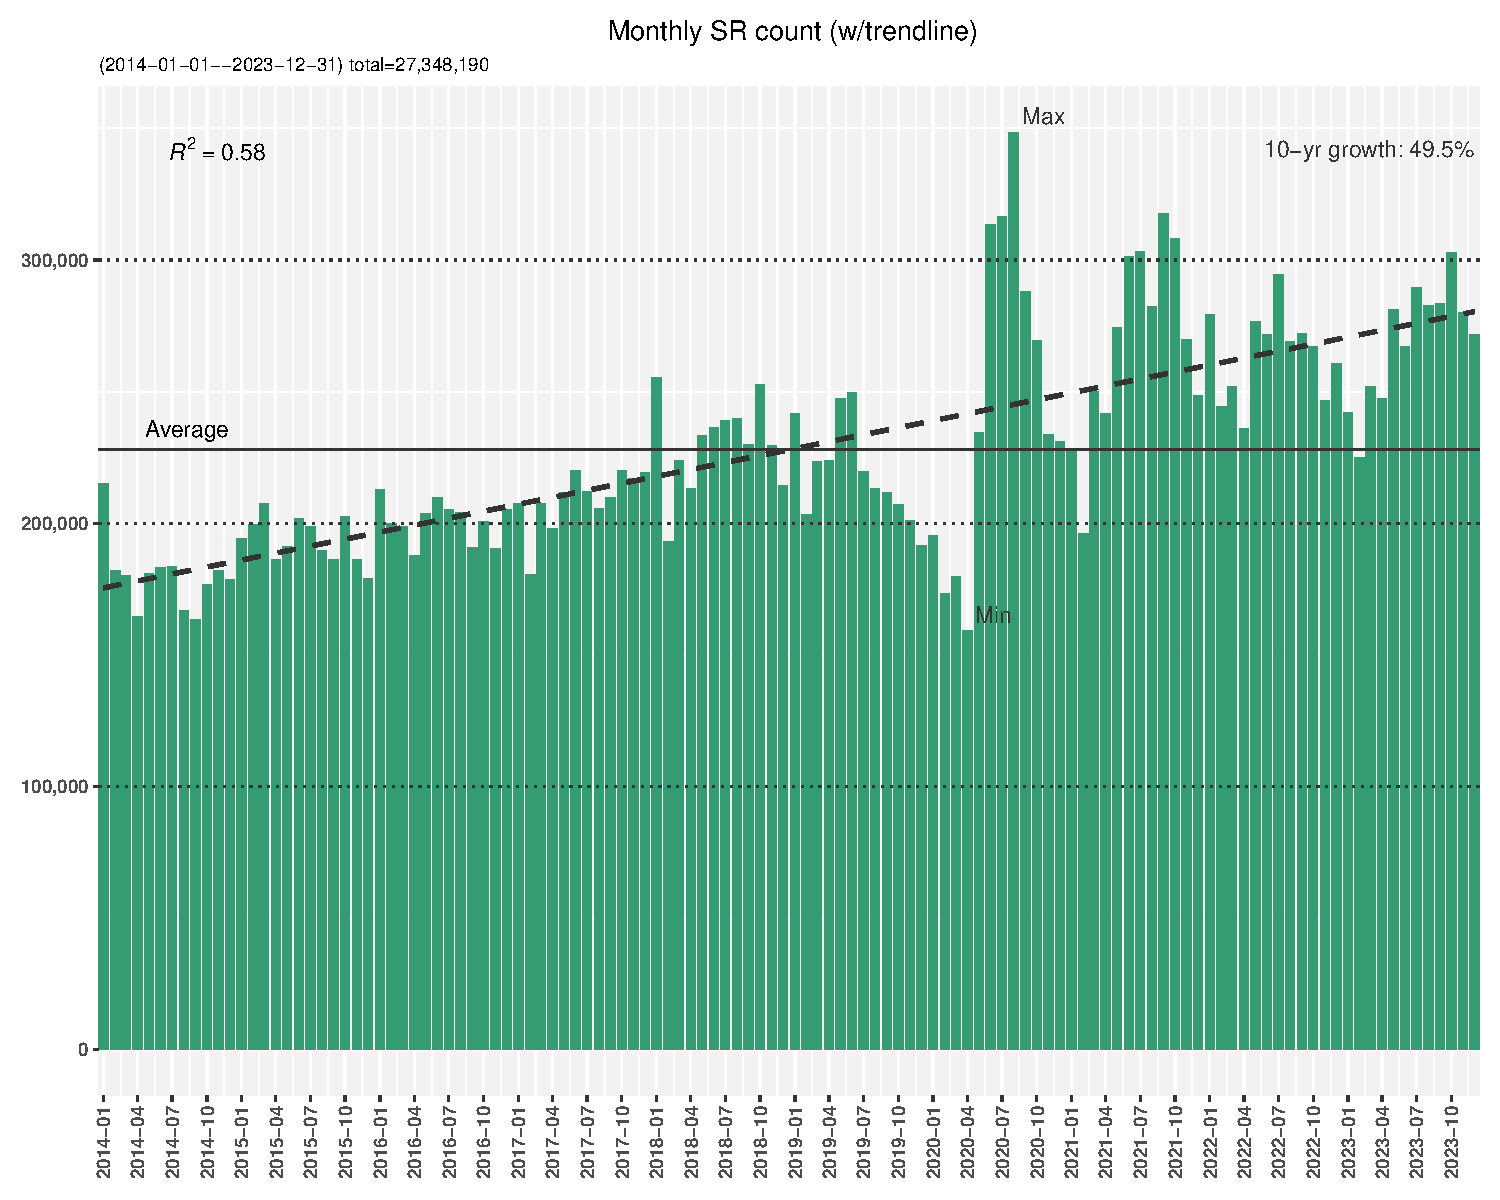
\includegraphics[width=0.8\textwidth]{10-year-trend-monthly.pdf}
  	\caption{10-year (2014-2023) Monthly SR Counts}
  	\label{fig:10-yr-monthly}
\end{figure}

We also looked at a 10-year period (2014-2023) to
observe system performance over a longer time-frame; see
Figure~\ref{fig:10-yr-monthly}. During that time-frame,
the number of 311 SRs grew by 50\%. The summer and early fall months 
make up all of the Top 5 SR counts by day.


\begin{table}[tbp]
    \centering
    \caption{Top 5 and Bottom 5 Days for SRs}
    \label{tab:top-10-counts}
    \begin{tabular}{@{}lll lll@{}}
      \toprule
      \multicolumn{2}{c}{Top 5 Days} & \multicolumn{2}{c}{Bottom 5 Days} \\
      \cmidrule(r){1-2} \cmidrule(l){3-4}
      Date & Count & Date & Count\\
      \midrule
      2020-08-04 & 24,415 & 2014-12-25 & 2965\\
      2020-08-05 & 19,560 & 2015-12-25 & 3247\\
      2023-09-29 & 17,962 & 2014-04-20 & 3287\\
      2020-07-05 & 16,916 & 2015-12-26 & 3405\\
      2020-06-21 & 15,883 & 2016-11-06 & 3419\\
      \bottomrule
    \end{tabular}
\end{table}


Table~\ref{tab:top-10-counts} summarizes the top 5 and bottom 5 days
in counts of SRs. The highest daily SR count, 24,415, occurred on
August 4, 2020, coinciding with the aftermath of Tropical Storm
Isaias, highlighting the system's critical role during crises. The
second-highest count, 19,560, was the following day, reflecting the
storm's continued impact. 
Conversely, the lowest daily SR count, 2,965, was on Christmas Day,
2014, with similar lows on other Christmas Days, indicating reduced
activity during major holidays. The data also shows fewer requests on
weekends, such as April 20, 2014 (Easter Sunday), and November 6, 2016
(a non-holiday Sunday).


\begin{figure}[tbp]
	\centering
	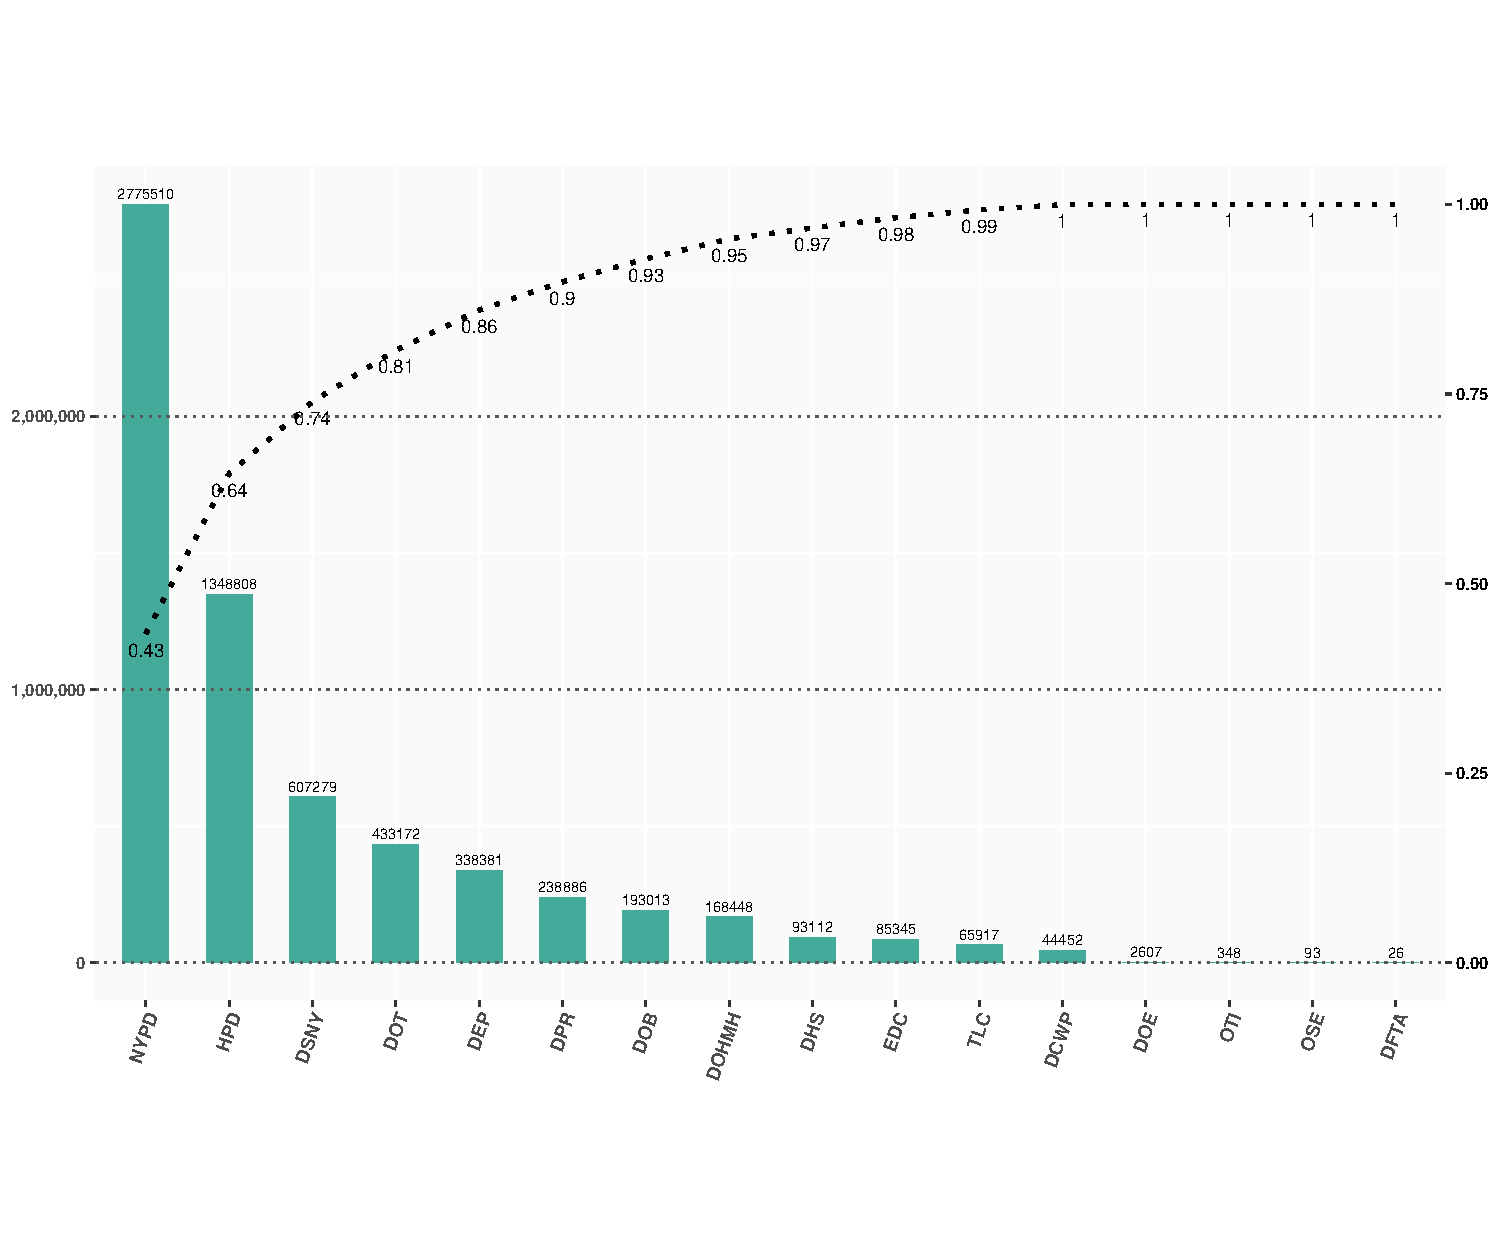
\includegraphics[width=0.8\textwidth]{SRs_by_Agency.pdf}
  	\caption{SR counts by Agency with Cumulative Percentage}
	\label{fig:SRcountbyAgency}
\end{figure}


Figure~\ref{fig:SRcountbyAgency} display the SR counts by agency with
cumulative percentage. Two important fields in this analysis are the
responsible NYC Agency and the type of complaint. Given the size of
the City of New York government, identifying the responsible agency
and the type of complaint is essential for pinpointing the accountable
party and troubleshooting discrepancies. This identification helps
determine whether an issue is specific to an agency or indicative of a
systemic problem. Although 311 SRs involve 16 different agencies, six
agencies account for 90\% of the complaints. These are the New York
Police Department (NYPD), Housing Preservation and Development (HPD),
New York City Department of Sanitation (DSNY), Department of
Transportation (DOT), Department of Environmental Protection (DEP),
and Department of Parks and Recreation (DPR).



\begin{figure}[tbp]
  \centering
  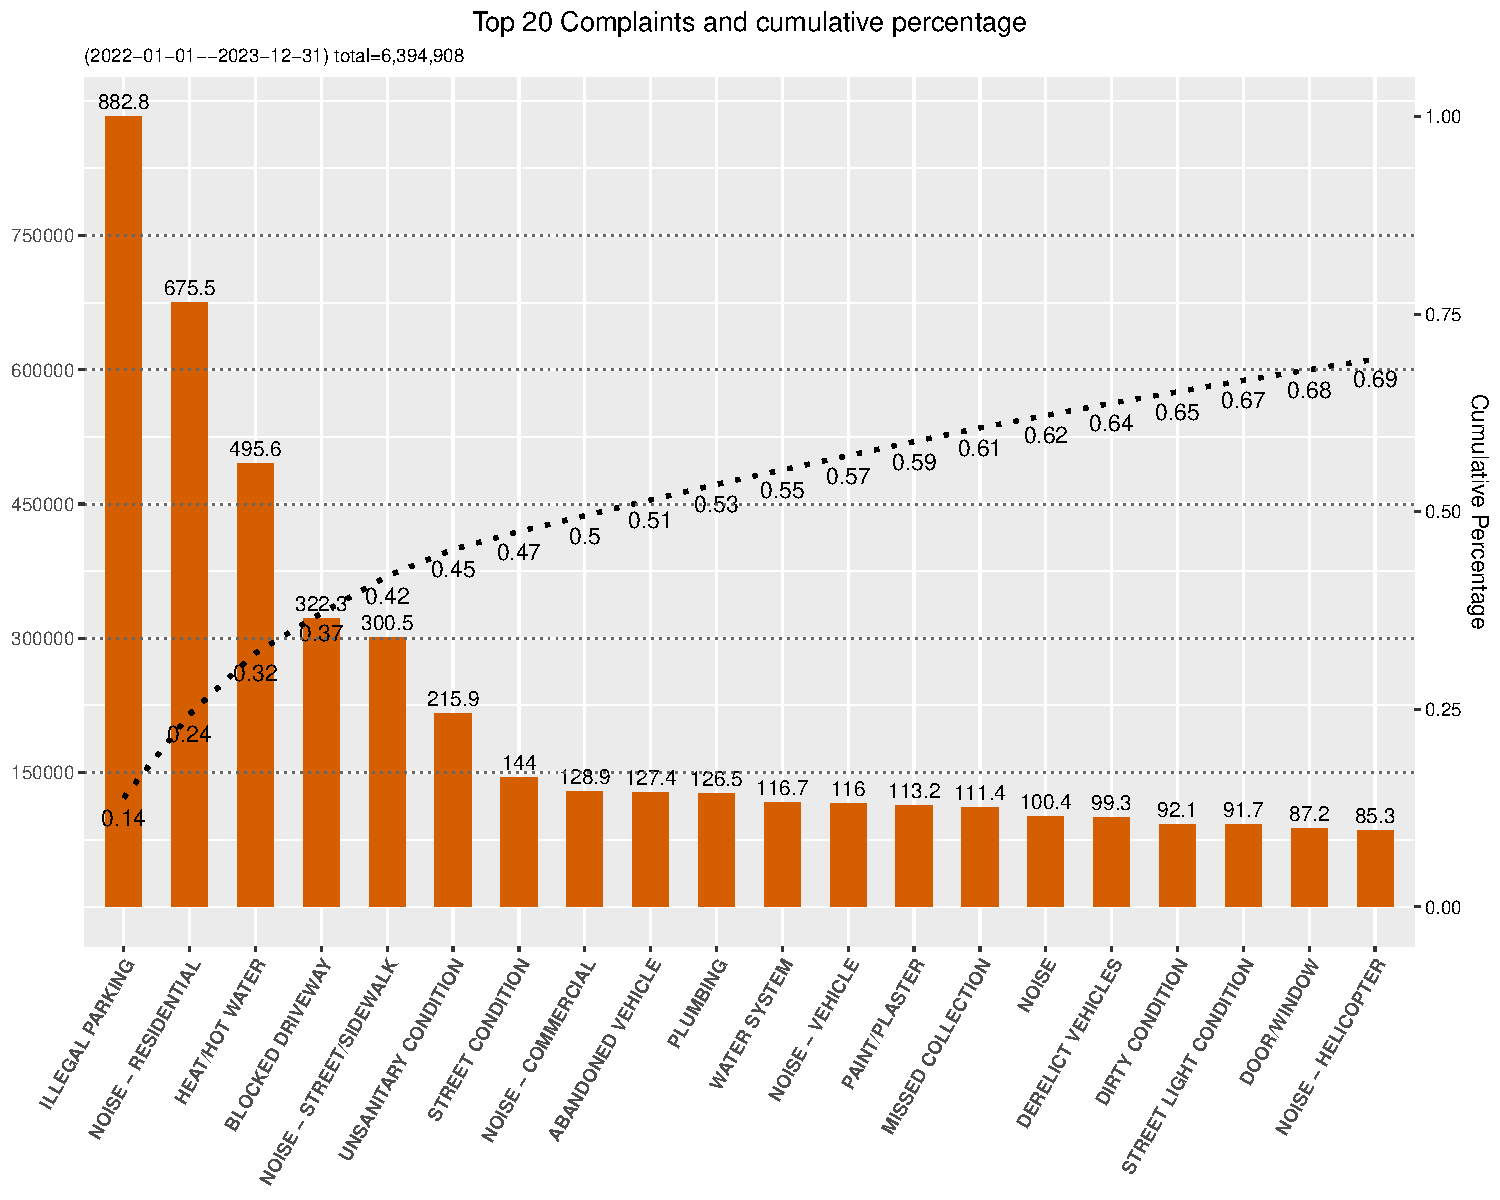
\includegraphics[width=0.8\textwidth]{SR_by_Complaint_Type.pdf} 
  \caption{Top 20 complaint\_type(s) and Cumulative Percentage} 
  \label{fig:SR_complaints}
\end{figure}

\begin{table}[tbp]
  \centering
  \caption{Noise-related complaints\_type(s) by count with Agency}
  \label{tab:noisecomplaints}
  \begin{tabular}{@{}lS[table-format=7.0,round-mode=places,
    round-precision=0]S[table-format=2.2,round-mode=places,
    round-precision=2]l@{}} % 'l' for left-aligned, 'S' for siunitx number alignment
    \toprule
    \textbf{complaint\_type} & \textbf{Count} & \textbf{Percentage} & \textbf{Agency} \\ 
    \midrule
    Noise - Residential        & 675502 & 10.56 & NYPD  \\ 
    Noise - Street/Sidewalk    & 300507 &  4.70 & NYPD  \\ 
    Noise - Commercial         & 128892 &  2.02 & NYPD  \\ 
    Noise - Vehicle            & 115956 &  1.81 & NYPD  \\ 
    Noise                      & 100413 &  1.57 & DEP   \\ 
    Noise - Helicopter         &  85345 &  1.33 & EDC   \\ 
    Noise - Park               &  16620 &  0.26 & NYPD  \\ 
    Noise - House of Worship &   2757 &  0.04 & NYPD  \\ 
    \bottomrule
  \end{tabular}
\end{table}

The distribution of complaint types skews toward a few select
categories, accompanied by a long tail. Figure~\ref{fig:SR_complaints}
shows that the top 20 complaint types account for 70\% of the total
220 different types. Notably, these top complaints include several
variations of noise-related issues, which collectively represent 22\%
of all complaints. When consolidated, noise complaints emerge as the
most frequently occurring type. Table~\ref{tab:noisecomplaints}
provides a detailed breakdown of noise-related complaint types by
count and responsible agency. The most common noise complaint is
``Noise - Residential,'' with 675,502 complaints, accounting for 10.56\%
of all service requests, and primarily handled by the NYPD. Other
significant noise complaints include ``Noise - Street/Sidewalk"
(4.70\%), ``Noise - Commercial'' (2.02\%), and ``Noise - Vehicle"
(1.81\%), all managed by the NYPD. Additional categories such as
"Noise - Helicopter'' (1.33\%) fall under the jurisdiction of the EDC,
and ``Noise'' (1.57\%) is managed by the DEP. The prevalence of these
complaints underscores the critical role of the NYPD and other
agencies in addressing noise-related issues, reflecting the
significant impact of urban noise on residents' quality of life. This
data highlights the importance of efficient response and management
strategies to mitigate noise disturbances in New York City.




\section{Data Cleansing Issues} 
\label{sec:issues}
What is data cleansing?  Wikipedia 
\href{https://en.wikipedia.org/wiki/Data_cleansing}{Data Cleansing} offers a good definition. 

\begin{quote}\textit{Data cleansing or data cleaning is the process of detecting and 
correcting (or removing) corrupt or inaccurate records from a record set, 
table, or database and refers to identifying incomplete, incorrect, 
inaccurate or irrelevant parts of the data and then replacing, 
modifying, or deleting the dirty or coarse data.}
\end{quote}

Many quality criteria are required in order to process high-quality 
data. These include:

\begin{itemize}
	\item Data validation - this effort can span a number of criteria
	\begin{itemize}
		\item Mandatory fields: Certain data fields cannot be empty.
		\item Data-types: Certain fields must be of the correct type, e.g. numeric, 
		character, date, 5 numeric digits, etc. Typically these are specified 
		in a Data Dictionary.
		\item Domain compliance:  Many data fields must adhere to a specific 
		domain of values, e.g. statuses, state names, zip codes, gender. 
	\end{itemize}   
	\item Structural errors to include naming conventions, 
	 fields not in the Data Dictionary, or inconsistent data entry. For example 
	 intermixing blanks, spaces, NA, N/A, and \textless{}NA\textgreater{} 
	 all to indicate the absence of data.
	\item Redundant, unnecessary, or irrelevant fields
	\item Logical inconsistencies such as related fields that violate the 
	nature of that relationship, e.g. a ``due date'' that is before the ``created date''
	\item Accuracy versus precision
\end{itemize}

This analysis effort is to identify the presence of such errors; not to correct them. 
That effort would be undertaken only after an investigation as to the why
and how such errors came about, and a discussion as to whether or not it 
is even an ``error''. 



\section{Structural Issues}
\label{sec:structural}
Structural issues in the context of data cleansing refers to issues 
related to the how data is organized, formatted, or structured within a 
dataset. Structural issues can make it difficult to analyze the 
data effectively. Here are some characteristics of the 311 SR data set:

\begin{itemize}
	\item There are 47 columns of data for each row, exportable as a CSV file.
	\item There are four date fields (created, closed, updated, due).
	\item There are three borough fields; two of which appear to be duplicates.
	\item Two zip code fields, but not duplicates
	\item Seven street fields; one pair of which appear to be duplicates
	\item Two Police Precinct fields; not duplicates
	\item In addition to incident\_address, there are five additional location fields: 
	lat/long, street\_name, landmark, NY State plane, and Block \#
	\item One free-form text field, resolution\_description, which 
	supports 934 characters of input, including commas and special characters
\end{itemize}

\textbf{Issue: Fields not in the Data Dictionary} The 311 SR 
\href{https://data.cityofnewyork.us/api/views/erm2-nwe9/files/b372b884-f86a-453b-ba16-1fe06ce9d212?download=true&filename=311_ServiceRequest_2010-Present_DataDictionary_Updated_2023.xlsx}{Data Dictionary}
 identifies 41 data columns (fields) along with related information 
 for each column. However, when you download the data or 
 explore it via the online portal, you immediately note that there 
 are 47 columns (fields). The additional six fields are not addressed in the 
 Data Dictionary, but do and show up on the Column Manager widget
 as ``@computed\_region\_xxxx\_xxxx''. To some extent one can infer 
 what the these @computed\_fields are and how they are determined, but 
 it is not possible to know for certain. Most importantly, can these fields 
 be reliably used for analytical purposes?  These six fields are:

\begin{itemize}
	\item zip\_codes
	\item community\_districts
	\item borough\_boundaries
	\item city\_council\_districts
	\item police\_precincts
	\item police\_precinct 
\end{itemize}	

	
	
	
\section{Validating data types}
\label{sec:datatypes}
Fortunately, both the Data Dictionary and the portal column manager 
do a good job of indicating the data type. The following fields were 
checked for their specified data types:
	
\begin{itemize}
	\item created\_date, closed\_date, due\_date, and resolution\_action\_updated\_date: 
	All are all in proper date format.
	\item zip\_codes and incident\_zip: All are 5 numeric digits except 
	for two non-numeric entries for incident\_zip (``na'' and ``N/A'').
	\item x\_coordinate\_state\_plane \&  y\_coordinate\_state\_plane 
	(a NY State geo-location system): All are all numeric.
	\item latitude \& longitude: Both are numeric.
	\item community\_districts, borough\_boundaries, 
	city\_council\_district, police\_precinct, and police\_precincts: All are numeric.
	\item Free-form text fields that contain a ``,'' (e.g. incident\_address 
	\& resolution\_description) are properly enclosed in quotation marks.
\end{itemize}	

 

\section{Blank \& N/A data}
\label{sec:blanks}
Understanding the absence of data by field is an important factor 
when undertaking analysis. For example, if you wanted to see if the SRs were
closed before or after their due\_date, you would be challenged 
as 99.57\% of the due\_date field is blank. Which calls into 
question...are these missing values, or is the concept of a 
due\_date simply not applicable for the vast majority of SRs?

When counting the various fields for blank or N/A values, the fields appear 
to divide into three groups: \textbf{Mostly Empty}, \textbf{Partially Empty}, 
and \textbf{Few/None Empty}. he Mostly Empty category ranges from 93-99.9\% blank. 
It includes such fields as taxi\_company due\_date, pickup\_location, and 
landmark. The Partially Empty includes such fields as location\_type, borough, 
and cross\_street. And the Few/None Empty includes created\_date, 
complaint\_type, agency, and status. In some cases it may make 
sense to inquiry as to why some fields are frequently blank. Here is a graphic 
depiction of total empty (blank \& N/As) for each fields. You can see 
the natural grouping into the Most, Some, and Few categories 
in the stair-type visualization. 

\begin{figure}[tbp]
	\centering
  	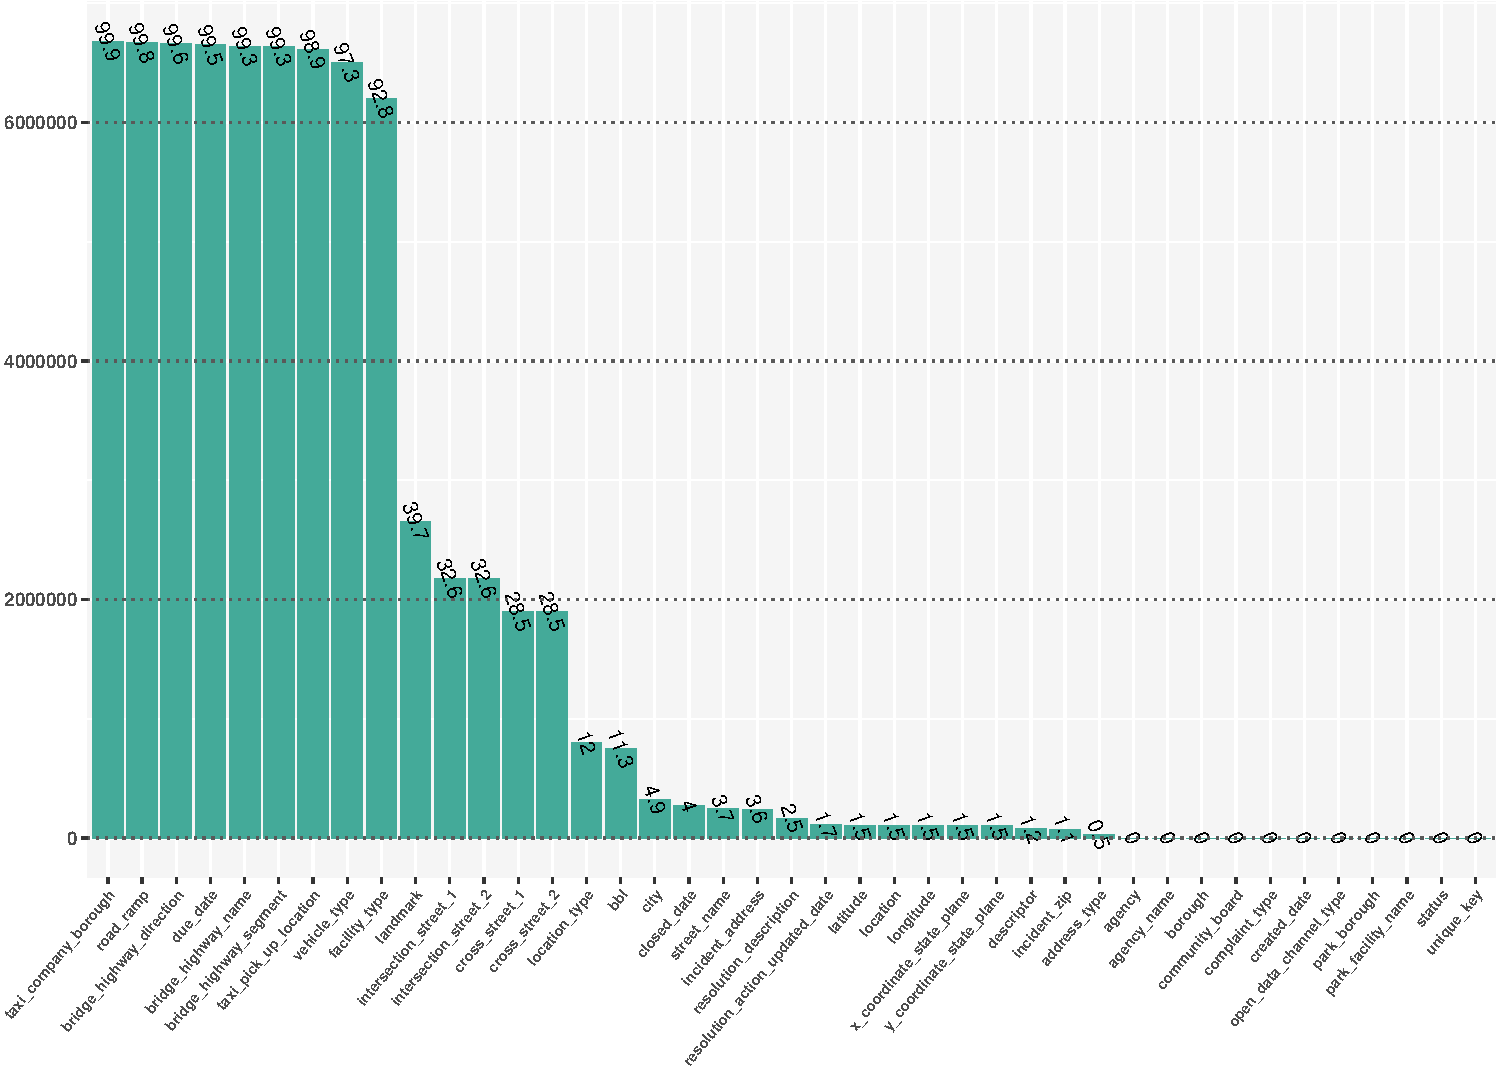
\includegraphics[width=\textwidth]{BlankFields.pdf}
	\caption{Number and Percentage of Empty/Blank Entries}
	\label{fig:blank_fields}
\end{figure}




 \section{Validating Data for Acceptable Values}
 \label{sec:domain}
 In this study, testing for invalid values revealed several issues 
 associated with select fields. Accordingly, an analyst needs to be 
 extra diligent if using these fields for analysis, and in all likelihood, 
 rows with invalid field values would  need to be removed from the 
 analysis. Here are some results.

\begin{itemize}
	\item Latitude and Longitude fields fell within the geographic 
	boundaries of New York City. 
	\item The unique\_key field was in fact unique.
	\item Many fields have a domain of acceptable values, often 
	determined from common usage or by examining historical 
	datasets. Unfortunately, these domains of acceptable 
	values are not specified in the Data Dictionary. These fields all tested as 
	compliant within their domain:
	\begin{itemize}
		\item address\_type
		\item status
		\item borough, borough\_boundaries, \& park\_borough 
		\item data\_channel
		\item vehicle\_type
		\item city\_council\_district
	\end{itemize}	
\end{itemize}

\subsection{Issues with Zip Codes}
\label{sec:zipcodesissues}
 Unfortunately some fields proved to be  problematic when comparing 
 the values to a domain of legal values. For example, all zip codes 
 (two fields: zip\_codes and incident\_zip) should be valid as defined 
 by the USPS database which contains 37,946 valid zip codes. However,
 the computed field zip\_codes proved problematic with 
58\% (3.6 million) of the field entries being invalid. Even the 
field incident\_zip while having only .07\% invalid entries, exhibited
4163 such errors. The breakdown of the invalid entries in the zip\_code, sorted by 
Agency shows that the distribution by percentage almost precisely 
mirrors the overall breakdown of SRs by Agency, potentially indicating
a systemic problem.
	
\subsubsection{Case Study: Noise Complaints by Zip Code}
\label{sec:case-study-zip-codes}
\textbf{Scenario:} The NYC Office of Nightlife (ONL) wants to 
know ``What are the top 10 zip codes for Noise Complaints (all 8 types) 
over the last two years?'' The intent is to assess the impact of the 
recent NYC effort promoting a vibrant nightlife 
in NYC while seeking to ease strained relations 
between bar and club owners. Let's assume that this analysis 
uses the zip\_codes field, one of the (six) 
computed fields that has shown to have validity problems. 
We then repeat the analysis with the incident\_zip field instead. Let's 
subject these two data sets to validation against the USPS zip code database.
	 
\begin{table}[tbp]
    \centering
    \caption{Comparison of Top Ten Zip Codes Lists}
	    \begin{tabular}{@{}lS[table-format=6.0,round-mode=places,
	    round-precision=0]c@{\hskip 0.5cm}@{}lS[table-format=6.0,
	    round-mode=places,round-precision=0]c@{}}
		\toprule
	 	\multicolumn{3}{c}{\textbf{zip\_codes}} & \multicolumn{3}{c}{\textbf{incident\_zip}} \\
	      \cmidrule(r){1-3} \cmidrule(l){4-6}
	      \textbf{Zip Code} & \textbf{Count} & \textbf{Valid?} 
	      & \textbf{Zip Code} & \textbf{Count} & \textbf{Valid?} \\
	      \midrule
	        11275 & 104556 & FALSE & 10466 & 104562 & TRUE \\
	        12420 & 27503 & TRUE & 10023 & 27972 & TRUE \\
	        12428 & 26564 & TRUE & 10031 & 25548 & TRUE \\
	        10935 & 25508 & FALSE & 10457 & 25066 & TRUE \\
	        10934 & 23448 & FALSE & 10453 & 24752 & TRUE \\
	        10931 & 22381 & TRUE & 10456 & 24751 & TRUE \\
	        10930 & 22121 & TRUE & 10452 & 22527 & TRUE \\
	        17613 & 21963 & FALSE & 10025 & 21705 & TRUE \\
	        10936 & 21707 & FALSE & 10458 & 21689 & TRUE \\
	        11606 & 21435 & FALSE & 10032 & 20622 & TRUE \\
	      \bottomrule
	    	\end{tabular}
 	\label{tab:zipcodes}
\end{table}

As indicated, six out of ten zip\_codes are invalid, which corresponds closely 
with what is observed in the overall dataset (58\%). Whereas the incident\_zip 
field is completely valid, again in-line with the overall incident\_zip 
validation percentage (99.04\%). If the analysis performed using the 
zip\_codes field were to be 	presented to the Director, ONL, the conclusion 
would be in error. 

\subsection{Issues with Police Precincts} 	
\label{sec:police-precincts}
A curious case also exists when examining the two nearly identical 
fields - police\_precincts and police\_precinct. Both of those fields 
are among the ``computed'' fields in the dataset. Using 
\href{https://www.nyc.gov/site/nypd/bureaus/patrol/precincts-landing.page}
{NYPD Precinct listings} it's possible to determine the valid 
police precincts; they are generally numeric or have numeric 
representations in the dataset. However, what we find is that 
both fields police\_precinct and police\_precincts  have  35\% 
invalid entries. Unfortunately, it's not the same invalid entries. For 
the police\_precincts field, there are 2,171,864 invalid entries 
(35\%)., a consequential number of errors. Similarly for the 
police\_precinct field, there are 2,171,778 invalid entries 
(also 35\%). 
	
\subsection{Issues with Community Boards}
\label{sec:communityboards}
Community Boards are an important aspect of NYC government. They are the 
most local, grassroots form of City government, and a vital connection 
between communities and elected officials and City agencies. Community 
Boards are used as a measure of City services throughout the five 
boroughs. In the 2022-2023 dataset there are 27,276 invalid community\_board 
entries which represents 0.43\% of non-blank data. The distribution 
of invalid Community Boards by Agency is not consistent with 
the overall SR Agency distribution. This indicates that there are likely 
specific issues at some key Agencies, in this case Taxi \& Limo 
Commission (TLC), Parks \& Recreation, etc. 

\subsection{Issues with Community Districts}
\label{sec:communitydistrict}
Another of the ``computed'' fields is community\_districts. Community Districts 
are the boundaries for the Community Boards, but unlike how 
Community Boards are an arm of the government of New York City, 
the Community District is used by the Department of City Planning 
(DCP) for purposes of environmental, socio-economic, and demographic 
purposes. It is a geographical division rather than a local 
government division. Due to how the community\_district data 
is formatted, it is not possible to establish validity. However, 
it is possible to determine that the dataset contains 72 unique 
entries, while there are only 59 valid Community Districts. 
	
\subsection{created\_date and closed\_date(s) -- Negative Duration}
\label{sec:negativeduration}
For the created\_date and closed\_date fields, you might 
expect that these two fields are automatically populated by the 
SR application software. Thus the created\_date is associated with setting an SR status 
to ``new'' or ``open''. And similarly when an SR's 	status is 
changed to ``closed''  the closed\_date would be 
populated. Unfortunately, that does not appear to be the case as
there are several anomalies with the various date fields.
	
\begin{itemize}
	\item SRs with a closed\_date that occurs before the created\_date.
 	\item created\_date(s) and closed\_date(s) in the far distant past.
 	\item created\_date(s) and closed\_date(s) that match to the second.
	\item A large number of SRs closed and created exactly at midnight 
	or exactly at noon. 
\end{itemize}
	
These date fields are important because citizens, NYC Government Officials, 
and NYC Agencies use these dates to measure the 
responsiveness for providing services. The measure of ``duration'',	 
of the response time of a 311 call is a closely 
watched, carefully scrutinized metric, both in terms of overall performance 
and with a geographical area. Duration, while not a field in the dataset, 
it is easily computed by closed\_date - created\_date.
	
Closed-before-Created:  There are 12,251 SRs that are closed before they 
were created, thereby generating a nonsensical ``negative duration''. 
While this is a small percentage overall (0.2\%) it can have significant impact 
on response time analysis. Here is a sample:
	
\begin{table}[tbp]
    \centering
    \caption{Largest and Smallest errors (days)}
	    \begin{tabular}{l l l r l}
	        \toprule
	        \multicolumn{5}{c}{\textbf{Largest errors (days) excluding 
	        extreme negative values}} \\
	        \midrule
	        \textbf{created\_date} & \textbf{closed\_date} & \textbf{duration} 
	        & \textbf{agency} \\
		        \midrule
		        2023-01-27 14:40:00 & 2022-01-14 14:40:00 & -378.0 & DOT \\
		        2023-01-18 10:06:00 & 2022-01-12 10:06:00 & -371.0 & DOT \\
		        2023-01-27 14:36:00 & 2022-01-22 14:35:00 & -370.0 & DOT \\
		        2023-01-11 11:10:00 & 2022-01-09 11:10:00 & -367.0 & DOT \\
		        2023-12-18 03:13:00 & 2023-01-16 13:10:00 & -335.6 & DOT \\
		        \midrule
		        \multicolumn{5}{c}{\textbf{Smallest errors (days)}} \\
		        \midrule
		        \textbf{created\_date} & \textbf{closed\_date} & \textbf{duration} 
		        & \textbf{agency} \\
		        \midrule
		        2023-06-28 07:07:31 & 2023-06-28 07:07:00 & -0.00036 & DOT \\
		        2023-06-29 09:10:20 & 2023-06-29 09:10:00 & -0.00023 & DOT \\
		        2023-01-12 06:50:13 & 2023-01-12 06:50:00 & -0.00015 & DOT \\
		        2023-06-26 08:09:07 & 2023-06-26 08:09:00 & -0.00008 & DOT \\
		        2023-01-12 06:51:01 & 2023-01-12 06:51:00 & -0.00001 & DOT \\
		        \bottomrule
	    \end{tabular}
    \label{tab:combined_errors}
\end{table}
	
The largest errors are shown ``excluding extreme negative values''. We found 
eight SRs with extremely large negative durations (\textless{} -730), all containing 
an entry of ``1900-01-01'' as the closed\_date, which generates extremely large 
negative durations exceeding 44,601 days (122 yrs). That large of an anomaly 
can skew statistical results, even though the number of occurrences is 
small. According, these  SR rows are removed from the analysis. These 
extremely large negative duration SRs are all from the 
Department of Homeland Services (DHS) A visualization of the 
negative-duration SRs by Agency shows that this negative-duration 
issue is a DOT problem, where 95\% of these types of errors occur. 
	
\begin{figure}[tbp]
 	 \centering
 	 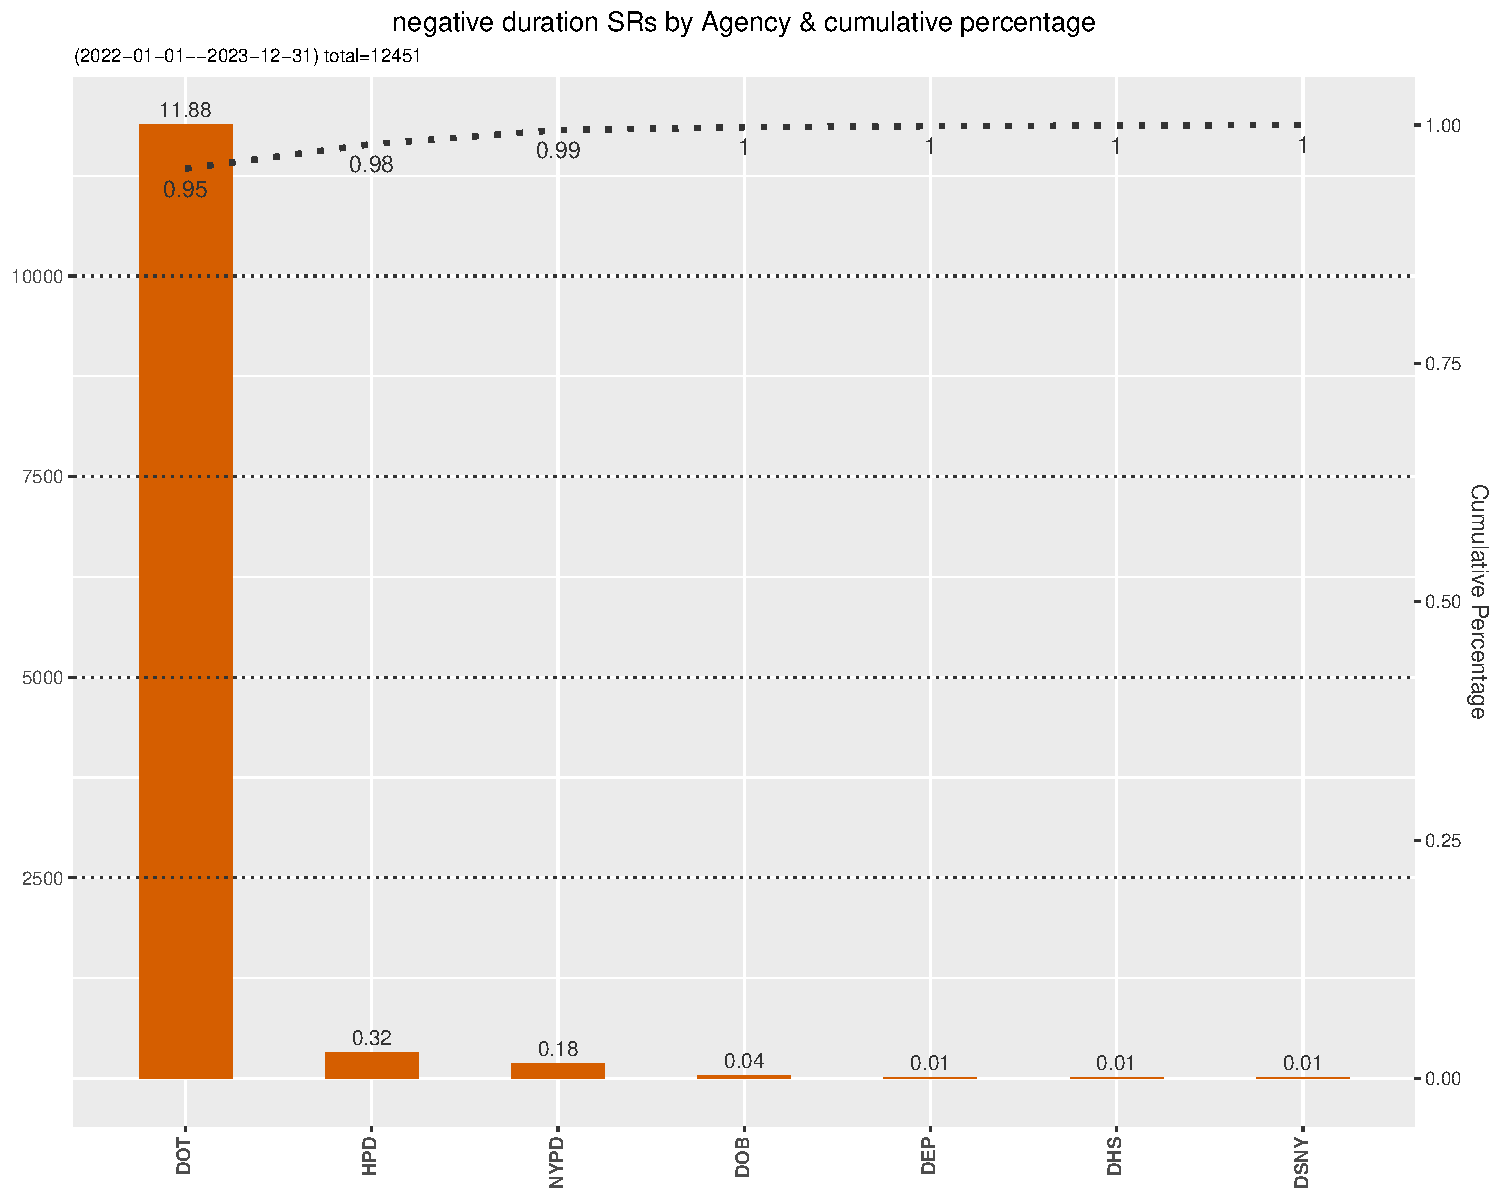
\includegraphics[width = \textwidth]{negative_duration_SR_barchart.pdf}
	  \caption{Negative Duration SRs by Agency}
	  \label{fig:negative-duration}
\end{figure}
	
This violin chart shows the broad spread of negative-duration SRs, albeit with 
the extremely large negative-duration SR removed. While there are few 
outliers, the magnitude of the negative-durations is troubling and can 
produce bizarre analytical results.
	
\begin{figure}[tbp]
 	 \centering
 	 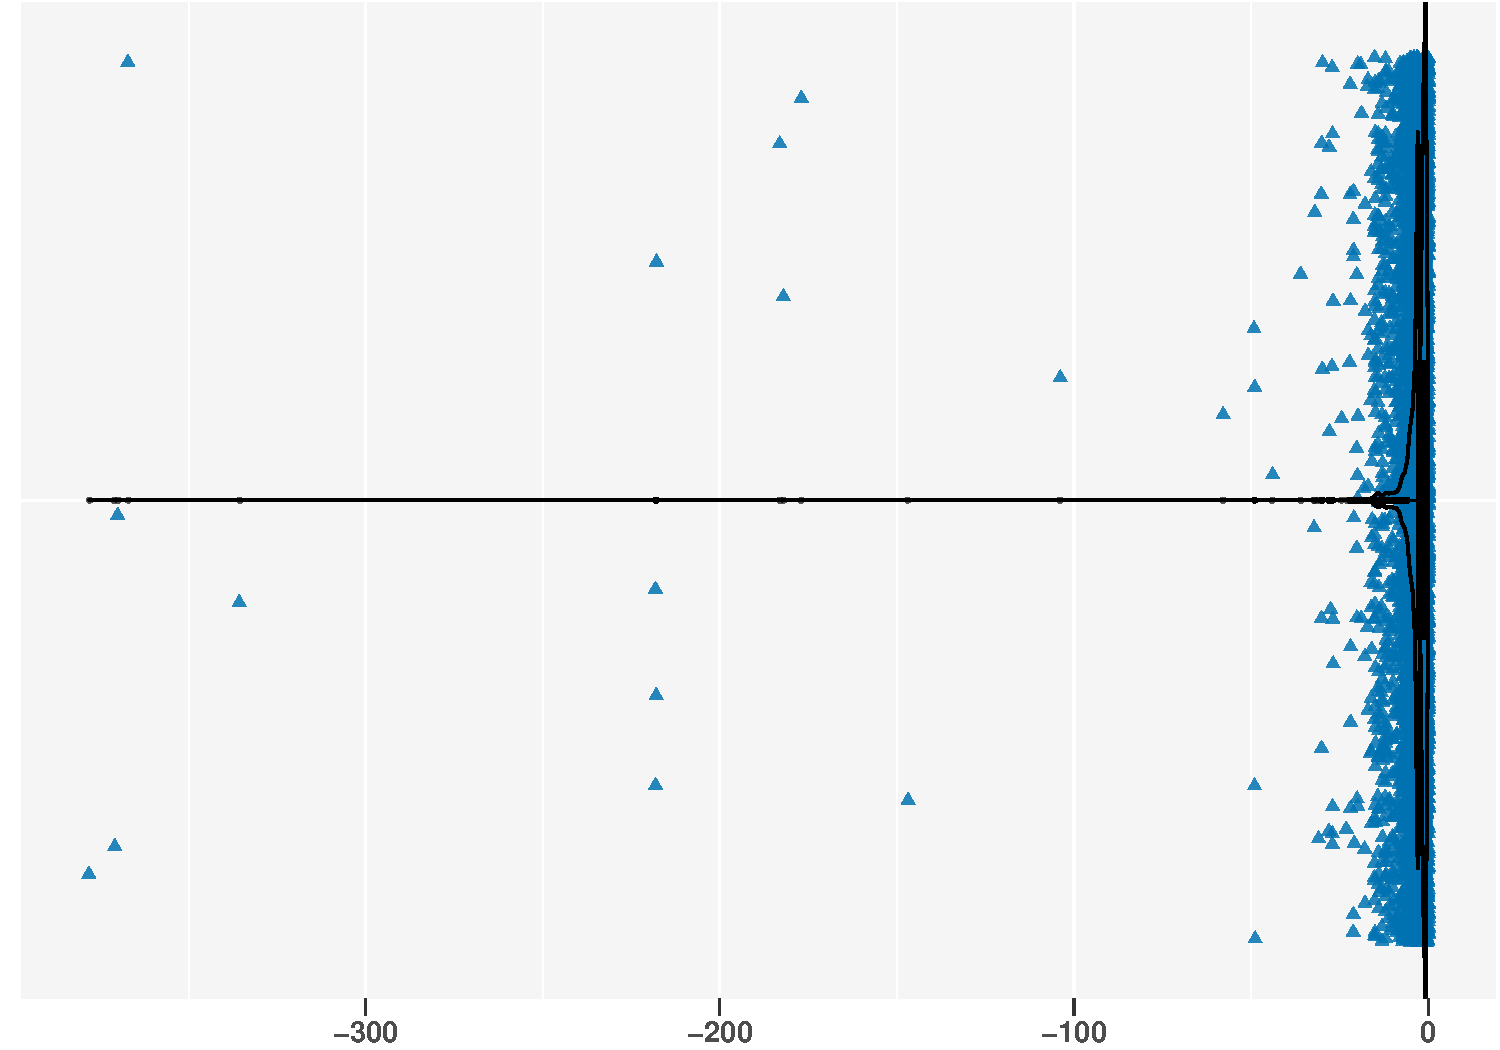
\includegraphics[width = \textwidth]{negative_duration_SR_violin.pdf}
	 \caption{Distribution of Negative Durations}
	 \label{fig:negative-duration-violin}
\end{figure}

\subsubsection{Case Study: Homeless Person Assistance}
\label{sec:homlessassistance}
\textbf{Scenario:} The Dept. of Homeless Services (DHS) wants to 
know ``How quickly are 311 calls for ``Homeless Person Assistance
resolved over the past two years?'' This is a typical request made by 
both the public and City government. It's a performance metric along 
the lines of ``How quickly is my Agency responding to ``critical'' 
requests, and does that performance vary by Borough, Zip Code, etc. 
As an analyst, this appears to be a routine effort: 
		
\begin{enumerate}
    \item Select data from 2022-2023 and filter the data by 
    complaint\_type = ``Homeless Person Assistance'' (yields 55,000 SRs)
    \item Compute a new field ``duration'' (closed\_date – created\_date)
    \item Take an average of the ``duration'' field == \textbf{Answer:  -4.8 days}  
\end{enumerate}
		
Clearly that answer is nonsensical. How did such a simple task result 
in an absurd answer? The answer lies in the computation of the ``duration'' 
field. As it turns out, there are eight DHS SRs that have a closed\_date 
of ``1900-01-01''. Each of those SRs creates a negative duration of -44,602 
days (-122 years). So just those eight SRs with extreme negative duration 
values is enough to drive the average of the 75,000 
Homeless Assistance SRs to a negative value, clearly incorrect.
		
In this case, the median is a better measure of central tendency than the average. 
And the median of the duration field is  0.2 days (approx 5 hrs). 
		
\begin{figure}[tbp]
 	 \centering
 	 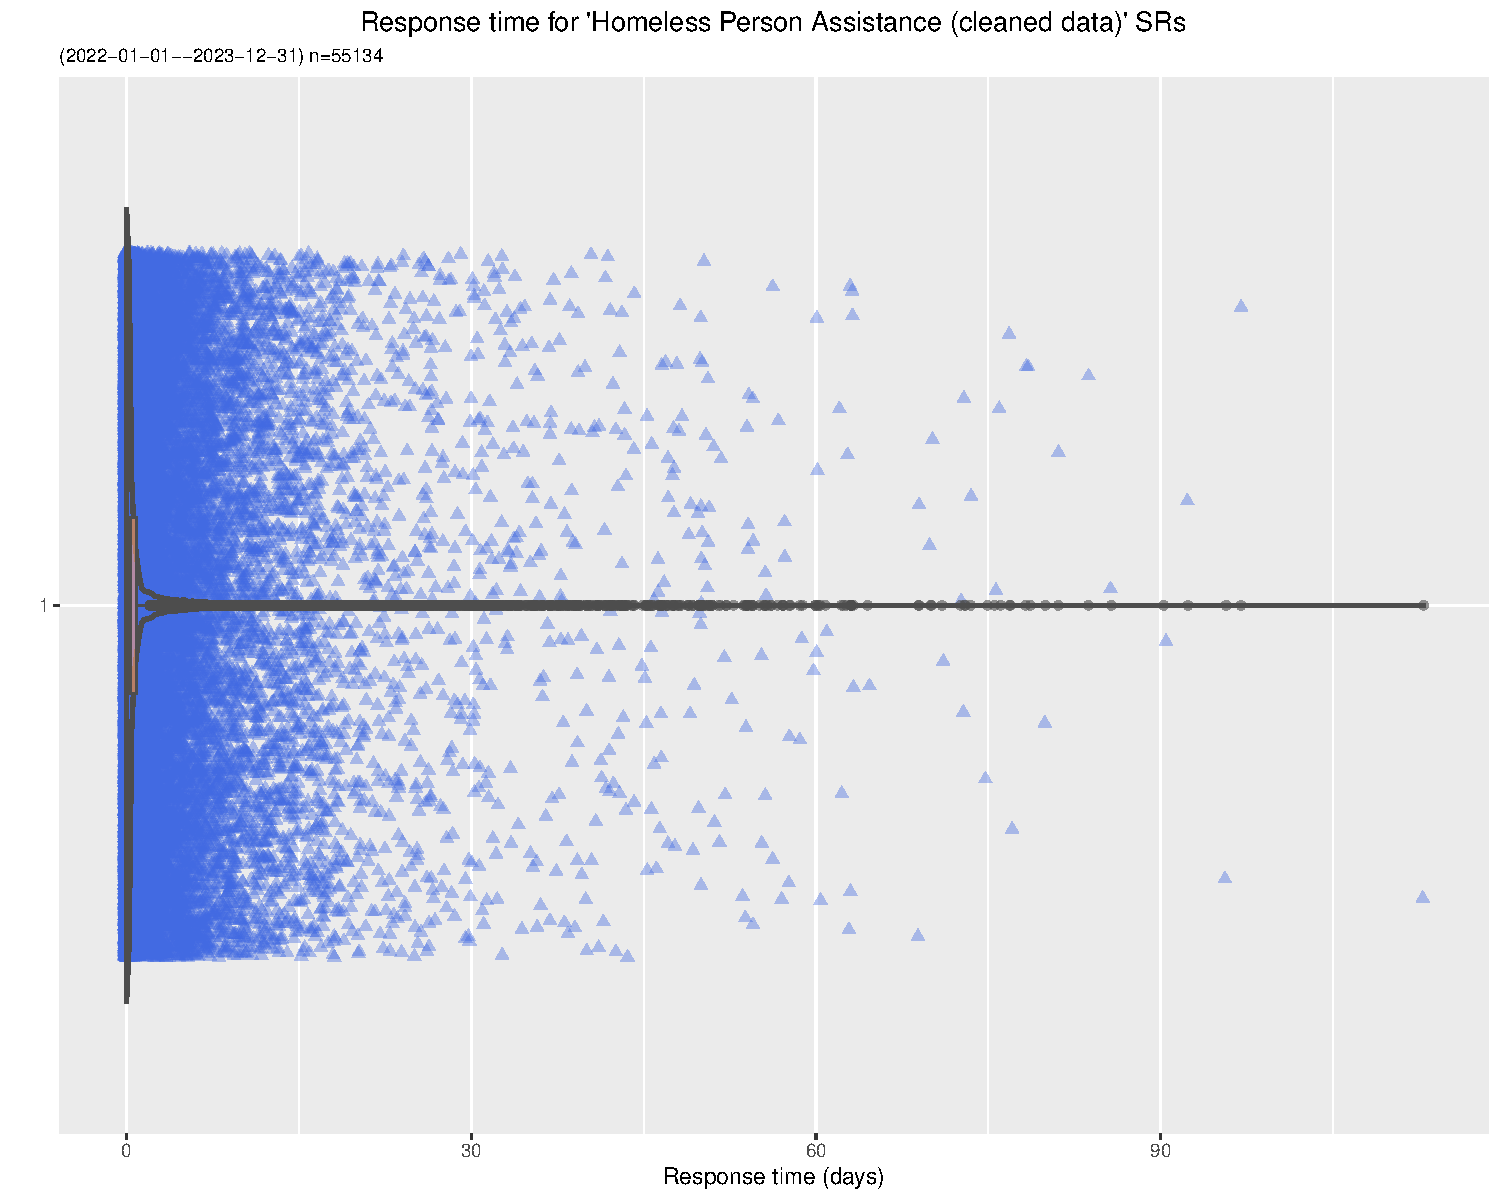
\includegraphics[width = \textwidth]{homeless_response_time_clean.pdf}
	 \caption{Homeless Assistance SR Durations}
	 \label{fig:homeless}
\end{figure}
		
\subsection{created\_date and closed\_date(s) --  Zero Duration}
\label{sec: zeroduration}		
A more serious and prevalent problem with closed\_date(s) 
occurs when the closed\_date and created\_date are exactly the same -- to 
the second -- which accordingly creates a \textbf{zero duration'}. Again 
this is nonsensical, and the presence of such zero durations can again 
severely distort analytics. There are 191,141 such SRs representing 3.1\% of 
all non-blank data. As shown in the chart 	below, 99\% of the 
zero duration SRs appear to predominately occur in five 
Agencies (Dept of Mental Health \&Hygiene, Dept of Transportation, 
Dept of Business, Dept of Sanitation, and Dept of Environmental Protection.) 
This is not in-line with the overall Agency distribution of SRs and indicates an 
Agency-specific issue, and the solution likely lies at those Agencies.
	
\begin{figure}[tbp]
	 \centering
	 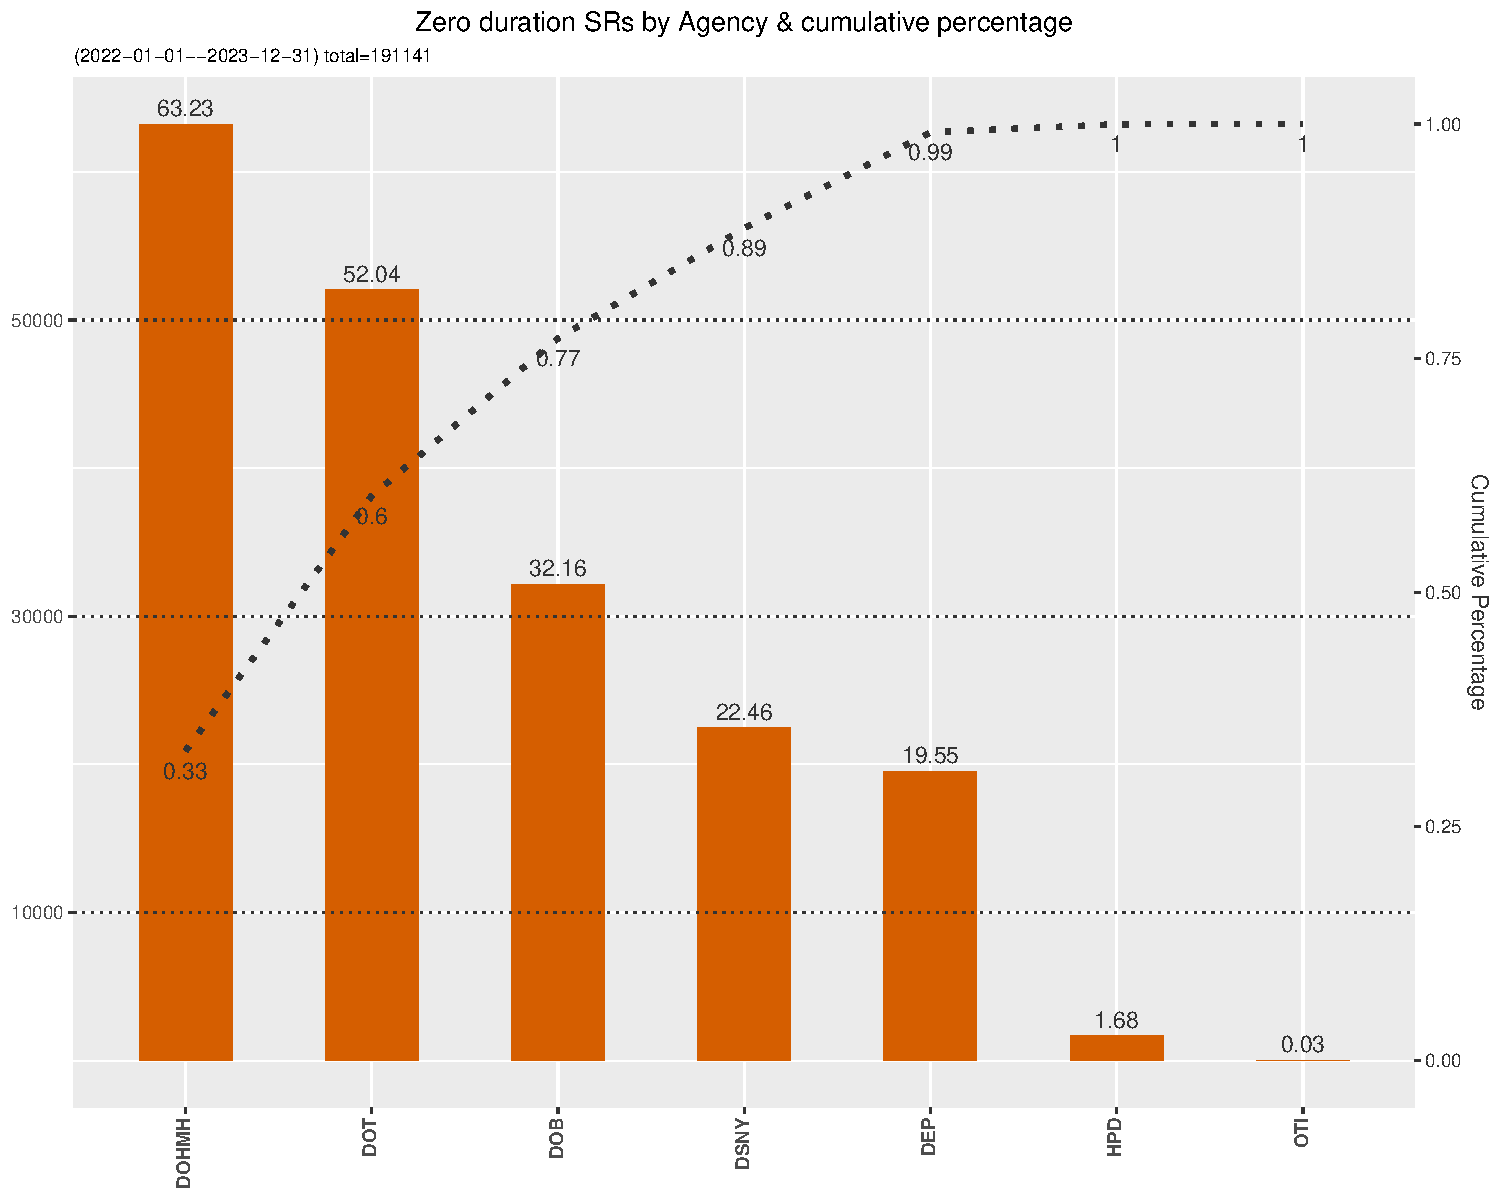
\includegraphics[width = \textwidth]{zero_duration_SR.pdf}
	 \caption{SRs with Zero Durations by Agency}
	 \label{fig:zero-duration}
\end{figure}	
		
\subsection{created\_date and closed\_date(s) -- Midnight \&Noon}
\label{sec:midnightandnoon}
Another problem discovered with the created\_date and 
closed\_date fields - there appears to be an unusually large number of SRs 
created or closed at exactly midnight (00:00:00) and exactly noon (12:00:00), 
to the second. The distribution of SR creation and closure largely follows the 
work-day clock with many SRs created during day-light hours, and 
fewer SRs 	created at night and the early hours of the morning. However, 
here there appears to be significantly greater numbers of SR closed exactly 
at midnight and exactly at noon, as well as a significant number of SRs 
created exactly at noon. Observations during this 2-year period include:
	
\begin{itemize}
	 \item There were 99,779 SRs created exactly at noon (12:00:00)
	 \item There were 235,347 SRs closed exactly at midnight (00:00:00)
	\item There were 105,505 SRs closed exactly at noon. 
\end{itemize}

One other way to visualize this anomaly is to look at the busiest day 
during this 2-year period (Friday, 2023-09-29). Then aggregate 
the created\_date(s) by minute (with seconds equal to zero), providing
a minute-by-minute look at SR creation. Here we see a clear 
spike at exactly noon (12:00), well beyond the 3\textsigma line.

\begin{figure}[tbp]
	\centering
	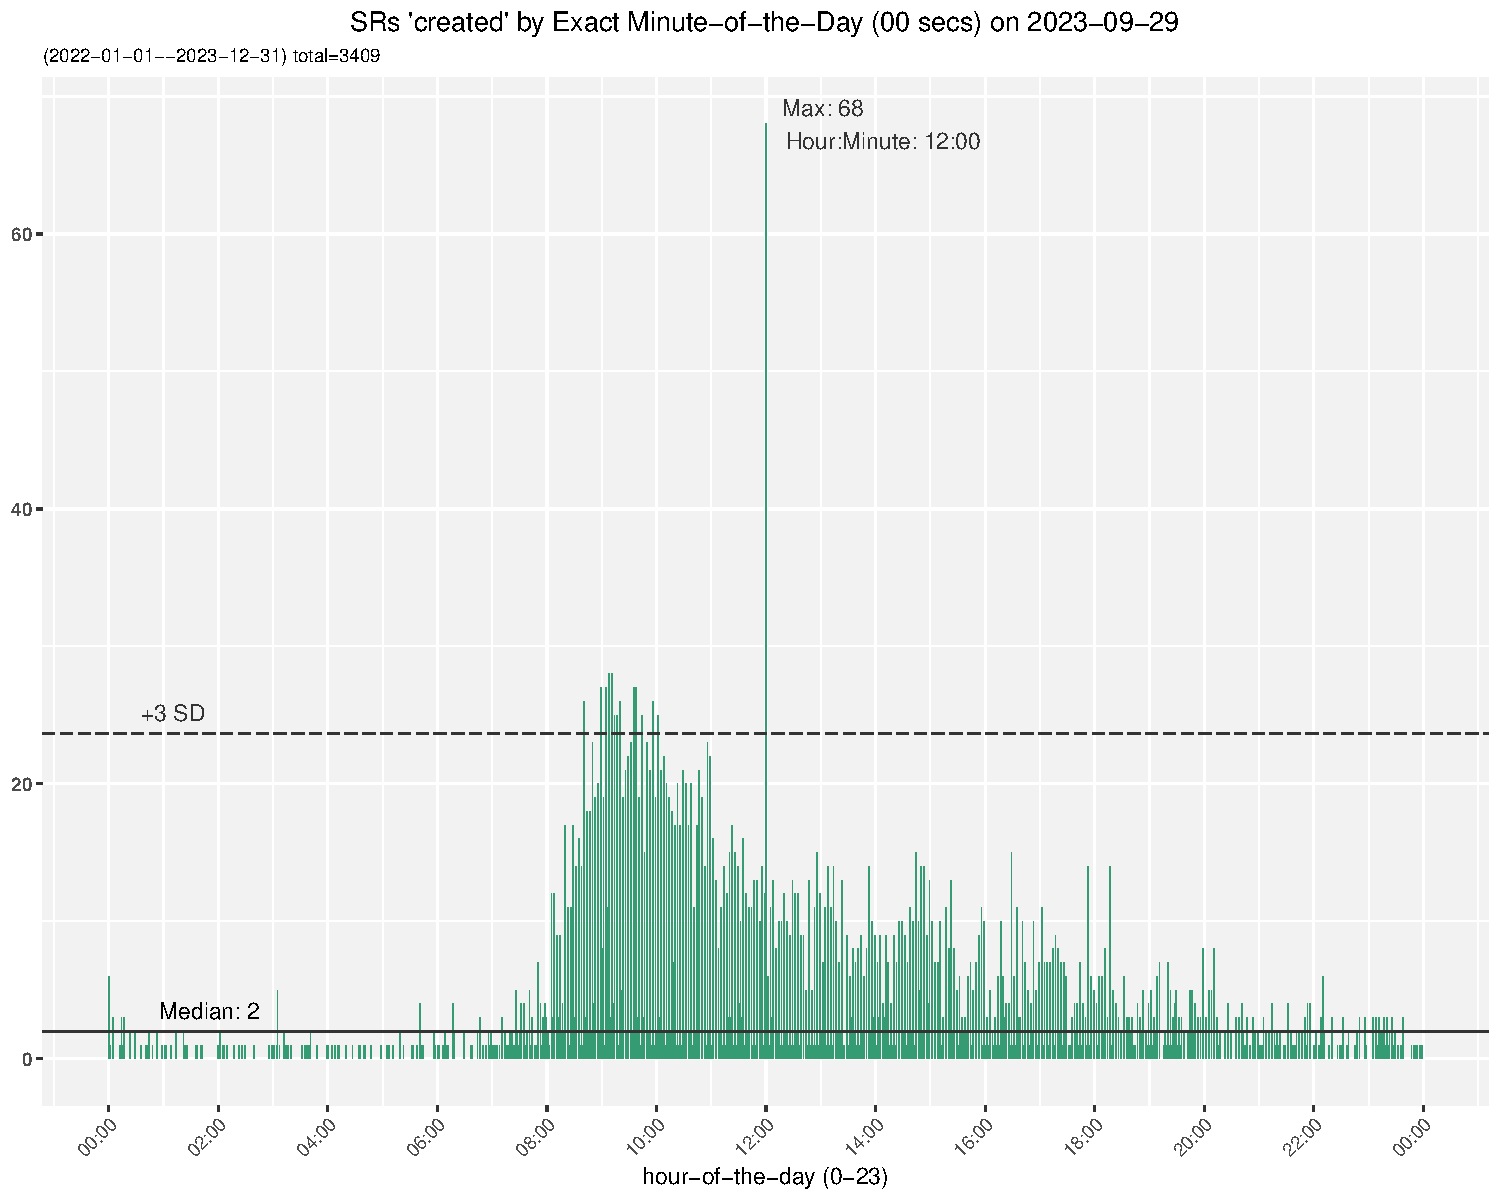
\includegraphics[width=\textwidth]
	{2-year-trend-SR_created_by_minute_of_busiest_day.pdf}
	\caption{SRs Created Minute-by-Minute on Busiest Day}
	\label{fig:busiestcreated}
\end{figure}	

As before, let's visualize this anomaly by looking at the closed\_date(s) 
on the busiest day during this 2-year study period (Friday, 2023-09-29). 
We aggregate closed\_date(s) by the minute (with seconds equal to zero). 
The chart highlights anomalies with spikes at 00:00:00 and 
12:00:00 respectively. 

\begin{figure}[tbp]
	\centering
	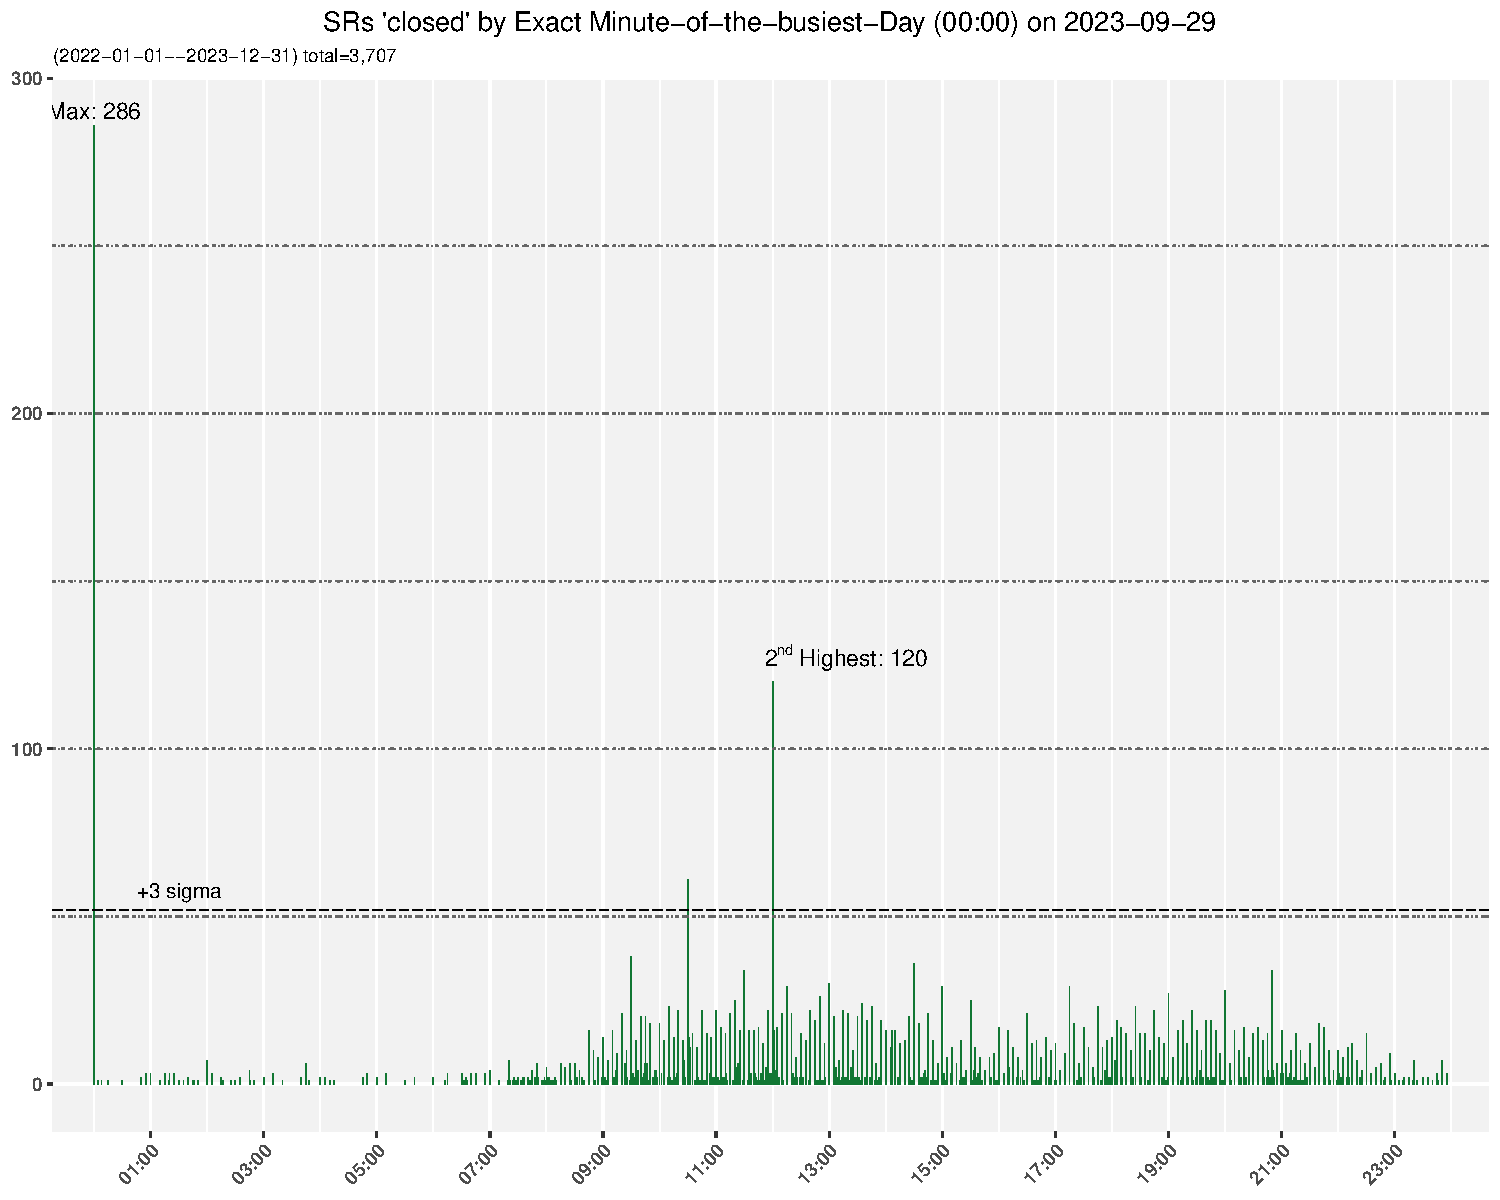
\includegraphics[width=\textwidth]
	{2-year-trend-SR_closed_by_minute_of_busiest_day.pdf}
	\caption{SRs Closed Minute-by-Minute on Busiest Day}
	\label{fig:busiestclosed}
\end{figure}	

These unusual patterns of created \& closed SRs at exactly the hours 
of midnight and noon likely indicates the presence of a bulk create/close 
software process that perhaps automatically ``closes'' 
(or ``creates'') a large number of SRs with a provided time-stamp of 
midnight (00:00:00) or noon (12:00:00). Again, such behavior will
distort the duration of these SRs. Looking at the distribution 
by Agency for the ``closed-exactly-at-midnight'' 
shows that \textgreater90\% of these suspect SRs come from just two 
Agencies - Dept. of Buildings (DOB) and Dept. of Sanitation (DSNY). 
	
\begin{figure}[tbp]
	\centering
	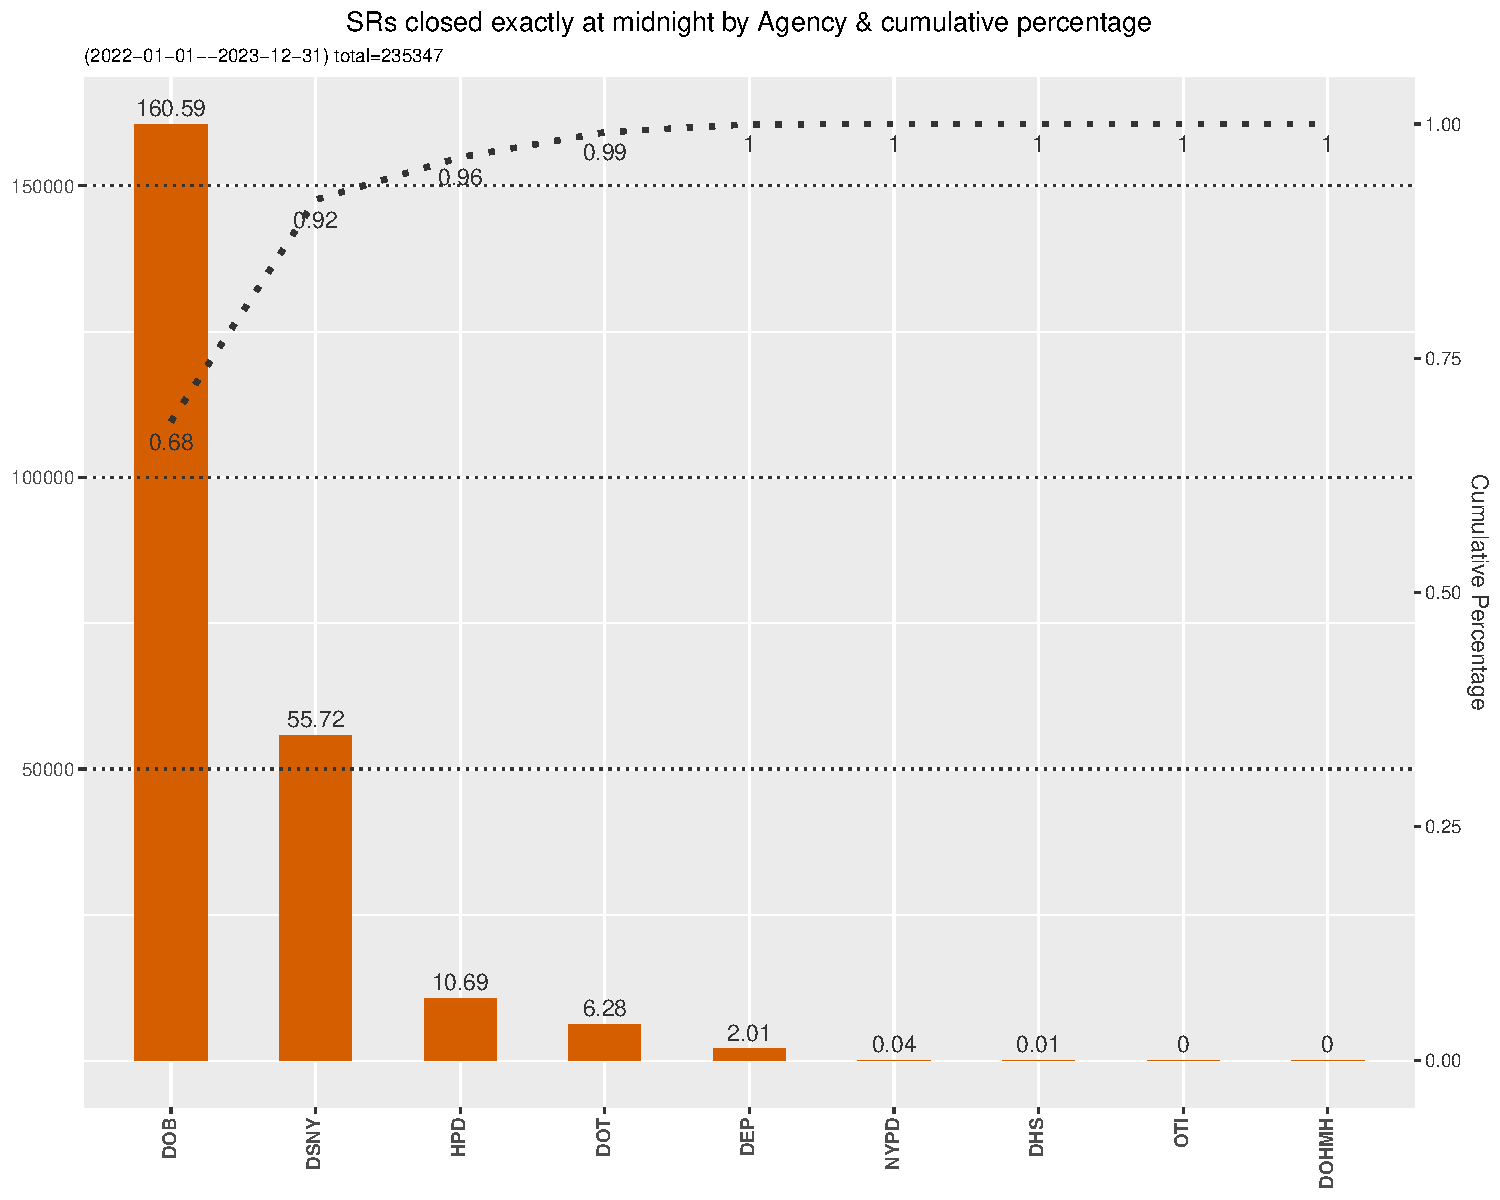
\includegraphics[width = \textwidth]{closed_at_midnight_chart.pdf}
	\caption{SRs Closed Exactly at Midnight by Agency}
	\label{fig:midnight-closed}
\end{figure}	

However, the ``SR closed at noon'' visualization shows that  a single 
Agency, DSNY, is responsible for \textgreater99\% of the 
SRs ``closed-exactly-at-noon''. 
	
\begin{figure}[tbp]
	\centering
	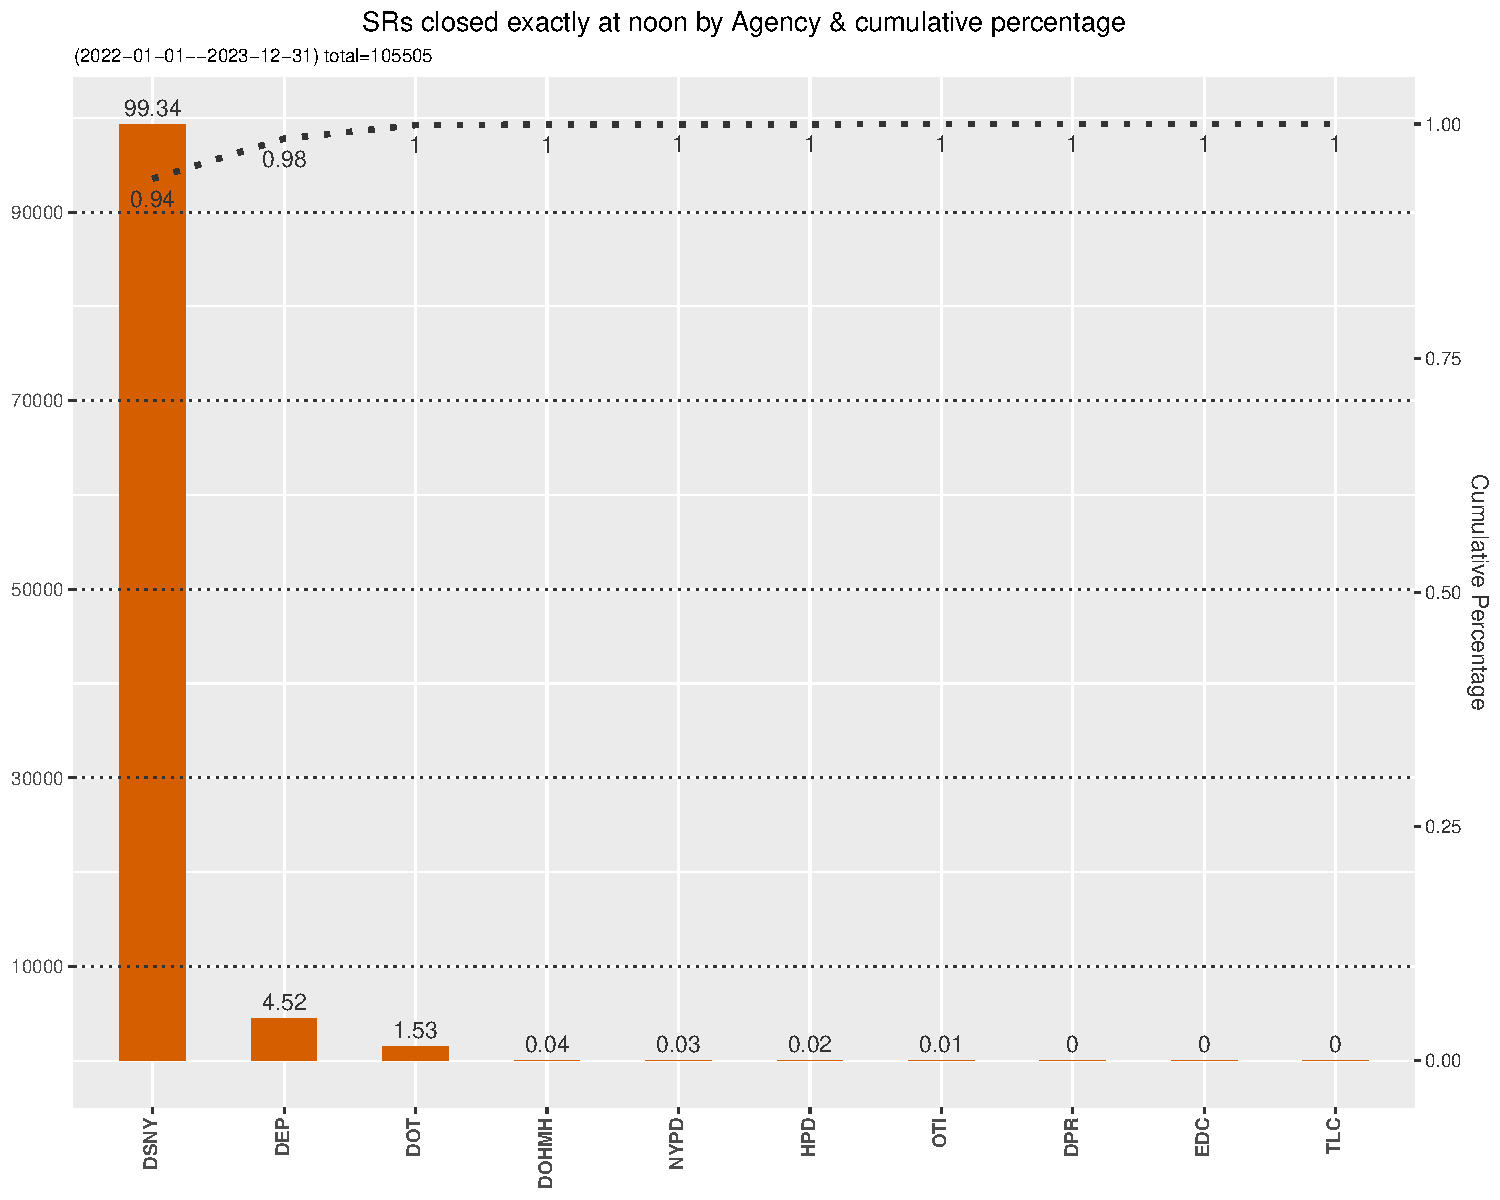
\includegraphics[width = \textwidth]
	{closed_at_noon_chart.pdf}
	\caption{SRs Closed Exactly at Noon by Agency}
	\label{fig:noon-closed}
\end{figure}	
		
\subsection{resolution\_action\_update\_date}
\label{sec: resolutionaction}
When an SR is updated, by any means on any field, the 311 software 
automatically populates the resolution\_action\_update\_date. 
Analyzing that field it becomes apparent that some of the SR updates 
are happening long after the SR is closed. There are a 
total of 7460 SRs that are updated \textgreater30 days and \textless{}730 
days after the closed\_date (to avoid infeasible dates such as 1900-01-01).
It is not known if this is normal behavior or an area that may 
require further investigation. 
	
\begin{figure}[tbp]
	\centering
	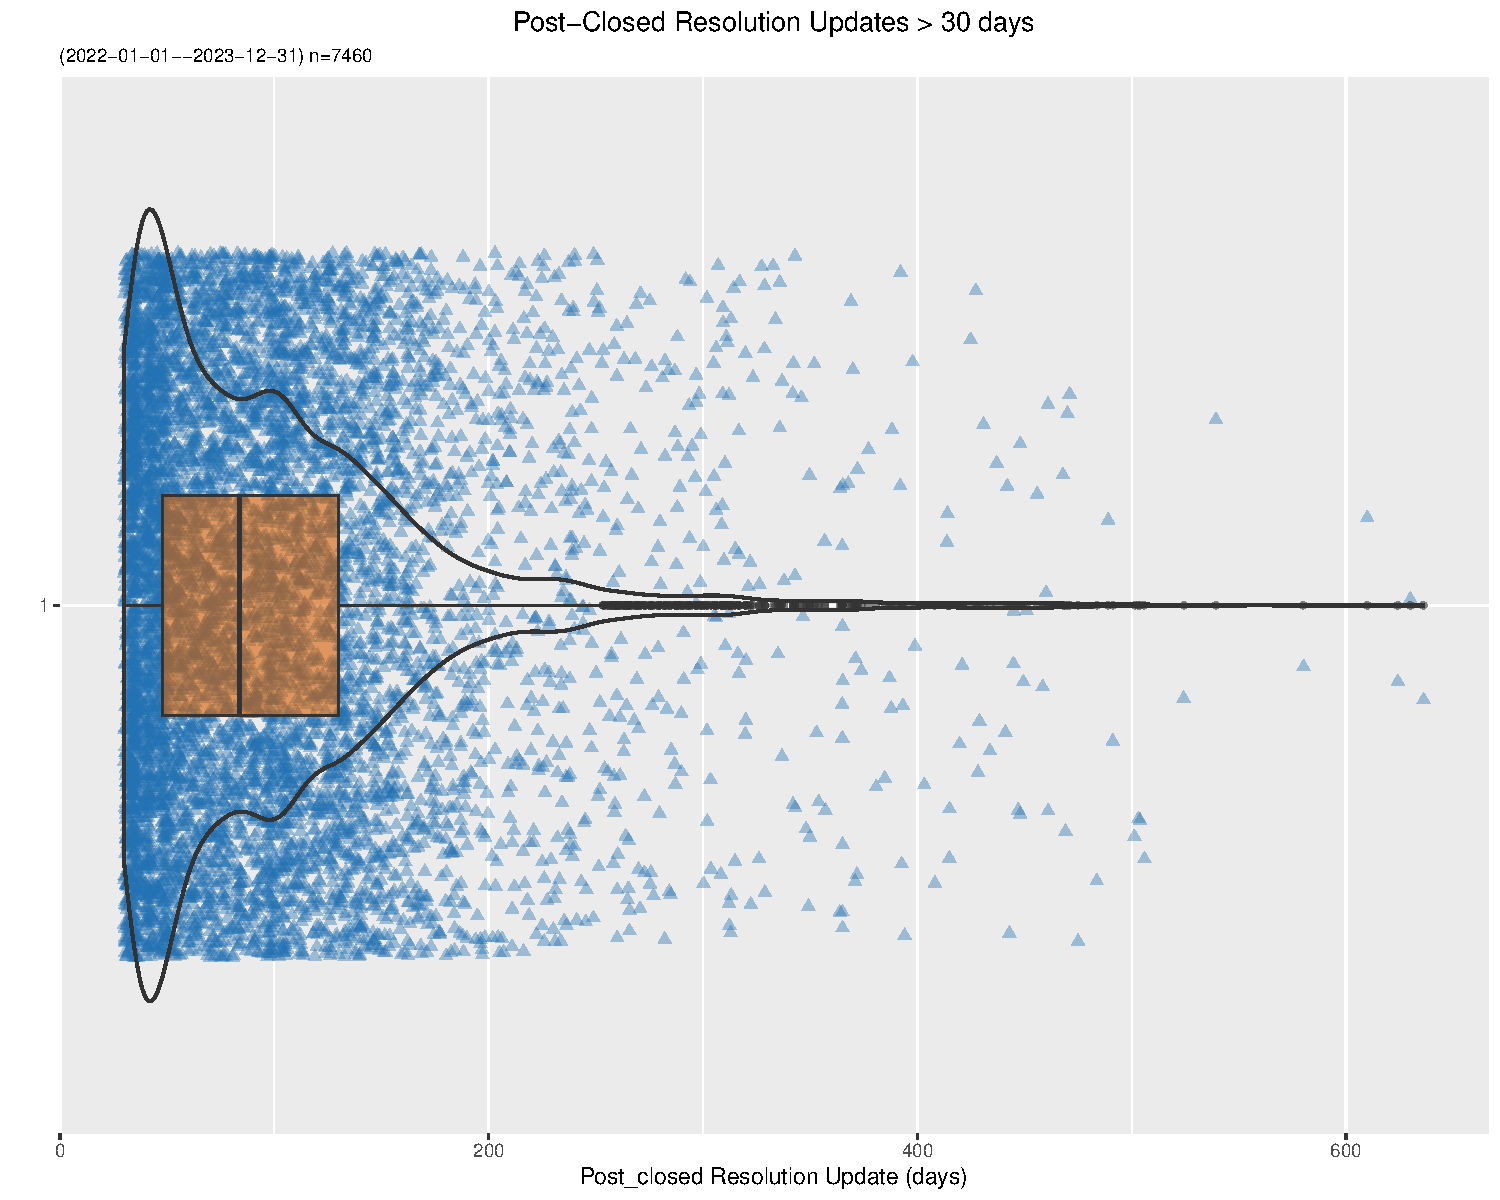
\includegraphics[width = \textwidth]{post_closed_violin.pdf}
	\caption{Post-Closed resolution\_action\_update\_date(s) 
	\textgreater30 days}
	\label{fig:resolution-violin}
\end{figure}		


	
\section{Accuracy and precision}
\label{sec:precision}
An area where the question of precision vs. accuracy arises is
with the Latitude and Longitude fields. Both the Longitude and 
Latitude fields are expresses as a 14-decimal 
number, e.g. 40.86769186022511. Also the Location field which is a 
straight concatenation of latitude and longitude). Given that 1 
degree of latitude at the equator is equal to 111.044736 kilometers, 
the ``1'' at the end of that number represents approximate 1.1104 nanometer 
or 1/1,000,000,000 of a meter. For reference a DNA molecule is 
approximately 2nm in width. Clearly the representation of 
the Latitude and Longitude fields are a classic case of 14-digit 
precision, but limited accuracy. 



\section{Redundant \& Duplicate fields}\label{sec:duplicates}
During this analysis, several redundant fields were observed. These 
fields should be examined further for possible consolidation.

\subsection{latitude \& longitude and the location fields}
\label{sec:latlong}
The location field is a pure concatenation of the latitude 
and longitude fields, with a comma and parenthesis 
added. The inclusion of the location field seems questionable 
as the data is arguably more difficult to extract than the 
two specific fields, especially for software programs. Example:  

\begin{itemize}
	\item  latitude: 40.768456429488
	\item  longitude: -73.9575661888774
	\item  location: (40.768456429488, -73.95756618887745)
\end{itemize}

\subsection{borough and park\_borough fields}
\label{sec:parkborough}
These two fields are 100\% matches; fully redundant.

\subsection{borough and borough\_boundaries fields}
\label{sec:boroughboundaries}
The borough field is a text field for the five New York City boroughs (Manhattan, Queens, 
Brooklyn, etc.). The borough\_boundary field is numeric with values 
from 1-5 corresponding to the five boroughs (Staten Island, Brooklyn, 
Queens, Manhattan, Bronx). When the borough\_boundary field is 
translated and compared to the borough field, there is a 
98.3\% match. And that is the problem with two ``near-duplicate'' 
fields; which field is correct when they disagree?

\subsection{borough and taxi\_company\_borough fields}
\label{sec:taxicompanyborough}
The two fields borough and taxi\_company\_borough might appear to be 
related. In fact, despite the names, the two data fields are nearly 
completely different with only 0.05\% matching. The mismatch is so 
high that it suggests the two fields are used very differently. This field 
is used exclusively by the Taxi \& Limo Commission which governs 
taxis and other cars for hire.

 \subsection{incident\_zip and zip\_codes fields}
 \label{sec:zipcodes}
 The zip\_code field is one of the six computed fields and its validity 
 has been explored in Section \ref{sec:zip-codes} and found to be 
 lacking with 55.55\% of the entries invalid according to the 
 USPS, while the companion zipcode field incident\_zip field had 
 an accuracy rate of 99.93\%. 

 \subsection{police\_precinct and police\_precincts fields} 
 \label{sec:police} 
Both the police\_precinct and police\_precincts are among the computed 
fields not cited in the Data Dictionary. Their usage however, is easy to 
discern. These two fields are near-duplicates with 99.94\% of the entries 
matching. Since the source of the fields and the underlying computational 
process are not know, it remains a challenge to determine which 
field is the ``right'' field to use. (The validity of these fields is 
covered in Section \ref{sec:police-precincts}.)

 \subsection{agency and agency\_name fields}
 \label{sec:agencyname}
 While not duplicates, these fields have a 1:1 correspondence.  The Agency 
 field contains abbreviations for the City agencies such as NYPD, DOT, 
 HPD, etc. The agency\_name field contains the full name of 
 the various organizations: New York Police Department, Department 
 of Transportation, Department of Housing Preservation and 
 Development, and so on. It seems redundant to include both.

\subsection{landmark and street\_name}
\label{sec:landmark}
The landmark field is listed in the Data Dictionary as ``Can refer to 
any noteworthy location, including but not limited to, parks, 
hospitals, airports, sports facilities, performance spaces, etc.'' Our analysis
found that was not the case. To be sure many of the entries in 
the landmark field do contain landmark names, e.g.``Pennsylvania 
Station'', ``La Guardia Airport'', etc., the vast majority 
of the entries are street names, e.g. ``Fenton Avenue'', ``Steinway 
Street'', ``Broadway''. These entries are similar to those in the 
street\_name field. And in fact, street\_name and landmark 
match 62\% of the time. While a high enough percentage of matching 
to be indicative of duplicate usage. Even the non-matches 
(excluding blanks) would appear to be matches except for minor 
spelling and nomenclature changes, e.g. ``NINTH AVE'' \& ``9 AVE''.

\begin{table}[ht]
    \centering
    \caption{Non-matches between 'street\_name' and 'landmark' fields}
	    \begin{tabular}{>{\raggedright\arraybackslash}p{5cm} >
	 	{\raggedright\arraybackslash}p{5cm}}
	 	\toprule
	      \textbf{street\_name} & \textbf{landmark} \\
	      \midrule
	        MACDOUGAL ST & MAC DOUGAL ST \\
	        NINTH AVE & 9 AVE \\
	        SIXTH AVE & 6 AVE \\
	        EAST FIRST ST & EAST 1 ST \\
	        FOURTH AVE & 4 AVE \\
	        SAINT LAWRENCE AVE & ST LAWRENCE AVE \\
	        MT HOPE PL & MOUNT HOPE PL \\
	        PENN STA & PENNSYLVANIA STA \\
	      \bottomrule
	    	\end{tabular}
    \label{landmark}
\end{table}
	
\subsection{cross\_street\_1 \& intersection\_street\_1 and cross\_street\_2 
\& intersection\_street\_2}
\label{sec:street1}
There are two sets of street pairs in the dataset in addition to 
the complaint address:

\begin{itemize}
	\item cross\_street\_1
	\item cross\_street\_2
	\item intersection\_street\_1
	\item intersection\_street\_2
\end{itemize}
	
These two pairs of streets are used to help identify the location of the 
reported incident, as it is common in New York City to provide the 
street address and the cross street, as in ``24 W 90th street between 
Columbus and Amsterdam''. For the majority of data rows, both 
pair of fields are populated and are duplicates; 88\% of 
cross\_street\_1 matches intersection\_street\_1. Similarly with
cross\_street\_2 exactly matches intersection\_street\_2.

\textit{(Note: Address standardization was applied to the street 
addresses using the R \emph{campfin} package. This was done 
to prevent generating a non-match between 
streets such as ``240 E 69\textsuperscript{th} ST'' and ``240 E 
69\textsuperscript{th} Street'' which are clearly the same address
but with formatting and spelling differences.)}

In addition to the matching/non-matching values, we encountered a number 
of \emph{near-matches}, cases where the 
cross\_street and intersection\_street are nearly identical, 
e.g. HARMON DR and HARMON RD. To identify these 
near-matches we measured the \href{https://en.wikipedia.org/wiki/Hamming_distance}
{Hamming Distance} between the two fields. The Hamming Distance is a 
measure of how many letters have to be changed in order for the two 
fields to match. For this analysis, we chose a Hamming Distance of 2. Here 
are the results for both cross\_street and intersection\_street.

\begin{table}[tbp]
    \centering
     \caption{Near-matches for cross\_street\_1, intersection\_street\_1}
     \label{tab:x1nearmatches}
		\begin{tabular}{l l l r}
	        \toprule
	        \textbf{cross\_street\_1} & \textbf{intersection\_street\_1} 
	        & \textbf{agency} & \textbf{hamming\_distance} \\
	        \midrule
	        WEST 168 ST    & WEST 167 ST           & DOT    & 1 \\
	        105 AVE        & 107 AVE               & DOT    & 1 \\
	        145 ST         & 150 ST                & DOT    & 2 \\
	        138 ST         & 139 ST                & DOT    & 1 \\
	        19 AVE         & 20 AVE                & DOT    & 2 \\
	        76 ST          & 79 ST                 & DOT    & 1 \\
	        67 ST          & 68 ST                 & DOT    & 1 \\
	        \bottomrule
	    \end{tabular}
\end{table}

\begin{table}[tbp]
    \centering
    \caption{Summary of cross\_street\_1 and intersection\_street\_1}
    \label{tab:summary1}
	    \begin{tabular}{l r r}
	        \toprule
	        \textbf{category} & \textbf{count} & \textbf{percentage} \\
	        \midrule
	        Matching                    & 5,637,182 & 88.15     \\
	        Both blank -- Matching      & 1,624,499 & 25.4      \\
	        Non-matching                &   757,726 & 11.85     \\
	        cross\_street\_1\_blank     &   222,232 & N/A       \\
	        intersection\_street\_1\_blank &   519,348 & N/A       \\
	        Near-match                  &       128 & 0.002002  \\
	        \bottomrule
	    \end{tabular}
\end{table}
\begin{table}[tbp]
    \centering
    \caption{Summary of cross\_street\_2 and intersection\_street\_2}
    \label{tab:summary_cross_intersection_2}
	    \begin{tabular}{l r r}
	        \toprule
	        \textbf{category} & \textbf{count} & \textbf{percentage} \\
	        \midrule
	        Matching -- non-blank      & 4,012,683 & 62.75     \\
	        Matching -- both blank     & 1,623,276 & 25.38     \\
	        Non-matching                &   750,543 & 11.74     \\
	        cross\_street\_2\_blank     &   222,788 & N/A       \\
	        intersection\_street\_2\_blank &   517,431 & N/A       \\
	        Near-match                  &     1,500 & 0.023456  \\
	        \bottomrule
	    \end{tabular}
\end{table}

\begin{table}[tbp]
	\centering
	\caption{Sample of near-matching cross\_street\_2 and 
     	intersection\_street\_2 (both non-blank)}
     	\label{tab:near_matching_cross_intersection_2}
	     	\begin{tabular}{l l l r}
	      \toprule
	      \textbf{cross\_street\_2} & \textbf{intersection\_street\_2} 
	      & \textbf{agency} & \textbf{hamming\_distance} \\
	      \midrule
	        227 ST         & 225 ST                & DOT    & 1 \\
	        65 ST          & 65 PL                 & DOT    & 2 \\
	        18 AVE         & 17 AVE                & DOT    & 1 \\
	        BEACH 110 ST   & BEACH 109 ST          & DOT    & 2 \\
	        88 ST          & 87 ST                 & DOT    & 1 \\
	        WEST 114 ST    & WEST 113 ST           & DOT    & 1 \\
	        5 AVE          & 4 AVE                 & DOT    & 1 \\
	      \bottomrule
	    	\end{tabular}
\end{table}


 \subsection{Shrinking file size by removing duplicates}
 \label{sec:filesize}
By removing duplicate and ``near-duplicate'' fields, it is possible to 
shrink the file size by 12.3\% which for this dataset equates to a 
reduction of 395 Mb. A smaller file size means faster downloads, 
less storage impact, as well as simplifying data analysis efforts.  
 
Below is a list of duplicate and near-duplicate fields. There are 
some challenges with these proposed deletions, mostly with 
the ``near duplicate'' fields.  So while the park\_borough is 
a complete duplicate of the borough field, the 
borough\_boundary field is only 98.3\% duplicate. Admittedly, 
loosing 1.7\% of the data in those two fields is quite small, however
for this large dataset that amounts to 110, 715 
non-matching occurrences. The authors  propose 
deleting the following fields from the data set.
 
\begin{itemize}
	\item agency\_name: Each row of data contains the agency field, 
	which is an abbreviation of the Agency's name. The agency\_name 
	abbreviations are clear, simple, and well understood.
		    
	\item park\_borough:  This field is a 100\% match with the 
	borough field. Removal of this field will not result in any loss of 
	data or data quality.
		    
	\item location:  The location field is a straight concatenation of 
	the latitude and longitude fields, with a comma and parenthesis 
	added. The data is a 100\% duplication of the latitude 
	and longitude fields. Removal of this field will not 
	result in any data loss.
		    
	\item police\_precinct: This field has a 99.95\% match with the 
	police\_precincts fields. We are unable to determine which field 
	is more correct, but feel that removal of one of the precinct fields 
	is prudent and would result in very minimal data loss.
		   
	\item borough\_boundaries (computed field): This field is one of 
	the six computed fields. It has a 98.3\% match with the borough 
	field.
		    
	\item cross\_street\_1 \& 2 and intersection\_street\_1 \& 2: These 
	two pairs of fields each have an 88\% match. We would recommend 
	deleting the two intersection\_street fields while acknowledging 
	some loss of data in doing so.
		     
	\item zip\_codes(computed field):  This field is one of the six 
	computed fields.  However, this field has error rate of 58\% and 
	as shown in the \ref{sec:case-study-zip-codes} can lead to 
	dangerous mistakes when used for analytical purposes. 
	We recommend deleting this field.
\end{itemize}
 	
Additionally, it would be worth investigating if certain data fields are 
in-fact useful, as the population of these fields is very, very scarce. For 
example, the taxi\_company\_borough field is 99.94\% 
blank. A similar situation exists for the road\_ramp field 
(99.75\% blank), the vehicle\_type field (99.71\%blank), and 
due\_date which is 99.62\% blank. There are several fields that are 
mostly blank: bridge\_highway\_direction, bridge\_highway\_name, 
bridge\_highway\_segment, and taxi\_pick\_up\_location...all 
of which have \textgreater99\% blanks. Most of those fields 
appear to used exclusively by the Taxi \& Limo Commission (TLC).   



\section{Data Dictionary Observations} 
\label{sec:datadictionay}
During this analysis, it became apparent that the  Data 
Dictionary could use an update. We found several discrepancies 
between the Data Dictionary and the actual data which can lead 
analytic efforts astray. 

===========================================
REVIEW BELOW HERE
===========================================

\begin{itemize}
	\item While the Open Data portal lists the basic data types of the 
	various fields, the Data Dictionary does not. Nor does it provide 
	meaningful information on the specifics of various fields, such 
	as constraints or domain of legal values. For example, the 
	incident\_zip field is specified as ``text''. That's probably not the 
	best definition, perhaps	``categorical'' would be more 
	appropriate with a description indicating that the data can 
	contain only numeric characters and is not subjected to arithmetic 
	operations. We found two instances with the zip\_code field 
	contained character strings (``na'', ``N/A''). 

	\item Domain of legal values as contained in the Data Dictionary 
	are incomplete. For example, the Data Dictionary indicates that 
	the status field has values of assigned, canceled, closed, or pending. 
	However, we found additional status values: in progress, started, 
	and unspecified. Additionally, we discovered no SRs with a status of 
	canceled. Similarly, the address\_type field is indicated to have 
	values address, blockface, intersection, latlong, and placename. We 
	discovered additional values of bbl and unrecognized. No values of 
	latlong were observed. Other fields suffer the same 	inaccuracies 
	(facility\_type, vehicle\_type, taxi\_pick\_up\_location, road\_ramp, city).
\end{itemize}



\section{Recommendations} 
\label{sec:recommendations}
Having identified a number of data cleanliness related issues with the 
311 Service Request (SR) dataset, what follows are a series of 
recommendations as to how to resolve these issues. Below are 
those recommendations;

\begin{itemize}
	\item First, and most importantly, the Open Data Team will need 
	to undertake a special effort to identify these data anomalies, confirm 
	the veracity of the issue, and engage with the appropriate Agency 
	Open Data Representatives to resolve these issues. That effort will 
	not be easy, fast, or cheap as in some software changes will likely 
	be required. Perhaps hardest will be working with the external City 
	Agencies that feed data to the 311 SR dataset, but are not using 
	the core 311 system. Integrations and API usage will need to be 
	investigated, and in many cases the changes required to correct 
	an issue will be on the source Agency side. Coordination and 
	mutual approval of any changes will be key. Strong support from 
	senior 	leadership will be a critical success factor.

	\item Secondly, standards will be to be identified, agreed to, and 
	commitment to support those standards must be obtained. For 
	example, what are the domain of legal values for certain fields, 
	especially those with identified issues?

	\item Obviously, many of the data integrity issues can be 
	resolved through rule enforcement by software. For example, the 
	software could easily prevent invalid values, such as zip codes, from 
	entering the system. Similarly for an entire range of data issues. One 
	key area is the created\_date and closed\_date which are frequently 
	cited when determining responsiveness of various Agency services. The 
	authors would argue that such dates should be driven by change 
	in ``status'', not manually entered. For example, the closed\_date 
	is captured when the SR ``status'' is changed to ``closed'', and 
	not manually entered. Such a change, along with many others, could 
	prevent errors such as negative and  zero durations which 
	significantly affect measurements of responsiveness. 
	
	\item The large spikes in SR closure and creation occurring at 
	midnight and noon, almost certainly point to an underlying automated 
	process from an external-to-311 Agency. Such processes again distort 
	the accurate capture of an SR duration. Data rule enforcement at the 
	software integration or API level should be investigated.

	\item One possible way to have software enforce certain data 
	standards, would be to move more non-311 Agencies to the core 
	311 software system. That system was completely upgraded in 
	2019, and should be (relatively) easy to expand to other 
	Agencies and usages.
	
	\item As noted, there are six ``computed'' fields in the data export 
	that are not identified in the Data Dictionary. While these fields may 
	be ``experimental'', they are nonetheless present in any data portal 
	presentation or export. As noted in this study, a number of those 
	computed fields suffer from data inaccuracies. It is difficult to know 
	what to recommend for these six field without further understanding of 
	their origin, computational method, or intended usage. We would 
	recommend updating the Data Dictionary at a minimum and 
	possibly hiding those fields from public display until such time as 
	their usage and accuracy can be ascertained.
	
	\item Removal of duplicate fields should be examined.  In some cases, such 
	as the borough and park\_borough fields, the duplication is 100\%. In 
	other cases, the duplication is in the 80-90\% range. These fields and 
	their usage/utility should be carefully examined to determine if 
	their inclusion in the 311 SR dataset is meaningful, adds value not found 
	in other fields, and should be removed or continued to be collected. Initial 
	analysis indicates that as much as 12\% size reductions are achievable 
	with the removal of duplicate fields. A more thorough review and 
	understanding of the fields would no doubt yield more savings. 
	
	\item Fields with extremely low data presence, such as taxi\_company\_borough 
	which is populated only 0.06\% of the time. Similarly for several other 
	fields evaluated in this study which have a high percentage of blank/unknown 
	values. If the presence of a small percentage of SRs with these fields 
	being populated is deemed useful and necessary, then so be it. But if 
	the usage of these fields is so diminished, then perhaps its inclusion 
	in the 311 SR dataset is not warranted.
	
	\item The Data Dictionary is in need of an upgrade and update. The last 
	revision is indicated at 6 March 2023, well over a year ago. 	As noted 
	in \textbackslash nameref: \nameref{sec:datadictionary} there are many 
	problems with the Data Dictionary, including domain values, absence of 
	the six ``computed'' fields, and inaccurate description of the usage of 
	several fields. Some of the Data Dictionary entries can be undertaken 
	immediately, which further revision should be addressed as part of 
	a deeper data clean-up initiative. 
	
	\item The excessive precision in the latitude, longitude, and location 
	fields is simply nonsensical.  We would recommend no more than 
	four decimal places (0.000X) which represents a distance of approximately 
	36.4 feet. Five decimals (0.0000X) represents 3.6 feet, which although 
	possible, would be an extremely sophisticated and accurate 
	geo-coding system. A 14 decimal number is simply a case of a lot 
	of precision with limited accuracy, and should be avoided.

	\item The 10 address-related address fields (incident\_address, 
	street\_name, city, intersection\_street\_1 \& 2, cross\_street\_1 \& 2,  
	landmark, road\_ramp, bridge\_highway\_segment, and 
	taxi\_pick\_up\_location should be in standard USPS format. There 
	are several software packages which can standardize addresses to 
	these standards. We believe such an effort should be automatically 
	applied to these fields at data entry. This step would also greatly 
	improve any underlying geocoding routines which 	may be used 
	to determine data values such as BBL, latitude, longitude, and New 
	York State X/Y-plane coordinates.
	
	\item The use of the value ``UNKNOWN'' , ``N/A'', ``NA'', and ``na'' when 
	entered directly as text into a field should be very carefully examined, 
	and in all likelihood prohibited.  There are some indeed a few 
	complaint\_type(s) where an ``N/A'' value is appropriate, such 
	as a consumer\_complaint about certain non-geocentric issues, such 
	as a travel agency or tax preparation service . But even in those cases 
	a value of ``N/A'' should be entered only via a drop-down menu 
	selection. During this analysis, there were far too many data 
	representations of missing data including: <N/A>, ``na'', `` ``, UNKNOWN, 
	and ``N/A''. It's challenging for analyst to have to account for so 
	the many different methods of representing empty or null data fields. 
\end{itemize}



\section{Protocol Suggestions} \label{sec:protocol}



\section{Discussion} \label{sec:discussion}

\bibliographystyle{asa}
\bibliography{ref}

\end{document}